% Compilação requerida: TeX Live com abntex2, babel-brazil, babel-english,
% amsmath, booktabs, tabularx, array, graphicx, microtype, hyperref, TikZ e
% pgfplots (TikZ libraries arrows.meta, positioning, shapes.geometric, fit e calc).
% Comando: latexmk -pdf -pdflatex="pdflatex %O %S" paper.tex
\documentclass[12pt,openright,twoside,a4paper,english,brazil]{abntex2}
\usepackage[utf8]{inputenc}
\usepackage[T1]{fontenc}
\usepackage{lmodern}
\usepackage{microtype}
\usepackage{amsmath}
\usepackage{booktabs}
\usepackage{multirow}
\usepackage{tabularx}
\usepackage{array}
\usepackage{graphicx}
\usepackage{tikz}
\usepackage{scalefnt}
\usetikzlibrary{arrows.meta,positioning,shapes.geometric,fit,calc}
\usepackage{pgfplots}
\pgfplotsset{compat=1.18}
\usepackage{hyperref}
\hypersetup{colorlinks=true,linkcolor=black,citecolor=black,urlcolor=black,
  pdftitle={Arquitetura de Soberania de Dados para Agentes de IA Pessoais: Um Modelo Local-First Baseado em Protocolos Descentralizados},
  pdfauthor={Pedro Henrique Almeida Prado de Oliveira}}
\DeclareUrlCommand\codigo{\urlstyle{tt}}
\newcommand{\micro}{\,$\mu$s}
\newcommand{\svnota}[1]{\begin{center}\fbox{\begin{minipage}{0.90\textwidth}\textbf{#1}\end{minipage}}\end{center}}
\titulo{Arquitetura de Soberania de Dados para Agentes de IA Pessoais: Um Modelo Local-First Baseado em Protocolos Descentralizados}
\autor{Pedro Henrique Almeida Prado de Oliveira}
\local{São Carlos}
\data{2026}
\instituicao{Universidade de São Paulo -- Instituto de Ciências Matemáticas e de Computação\par MBA em Inteligência Artificial e Big Data}
\tipotrabalho{Trabalho de Conclusão de Curso}
\preambulo{Trabalho de Conclusão de Curso apresentado ao Instituto de Ciências Matemáticas e de Computação da Universidade de São Paulo como requisito parcial para a obtenção do título de especialista em Inteligência Artificial e Big Data.}
% Orientadora confirmada pelo autor em 04/08/2026: Profa. Dra. Kalinka Regina
% Lucas Jaquie Castelo Branco (SSC/ICMC-USP). Perfil e pontos de apoio
% levantados em docs/thesis/orientacao/.
\orientador{Profa. Dra. Kalinka Regina Lucas Jaquie Castelo Branco}

\begin{document}
\pretextual
\imprimircapa
% A variante com estrela termina em \newpage (não \cleardoublepage), de modo
% que o conteúdo seguinte cai no *verso* da folha de rosto — que é onde a NBR
% 14724 exige a ficha catalográfica. Ver abntex2.cls, seção "Folha de rosto".
\imprimirfolhaderosto*
% A linha em branco acima é obrigatória: \imprimirfolhaderosto tem argumento
% opcional e, sem ela, o LaTeX consome o \begin{resumo} seguinte como argumento.

% ---------------------------------------------------------------------------
% Ficha catalográfica — NBR 14724 (elemento obrigatório), no verso da folha de
% rosto. O texto DEVE ser gerado pelo sistema da Biblioteca Achille Bassi
% (ICMC/USP) e colado aqui sem reformatar:
%   https://www.icmc.usp.br/institucional/estrutura-administrativa/biblioteca/servicos/ficha
% Trocar o bloco marcado pelo retorno do sistema. O aviso é intencionalmente
% visível no PDF para não passar despercebido na revisão final.
% ---------------------------------------------------------------------------
\begin{fichacatalografica}
% Transcrição literal do PDF devolvido pela Biblioteca Prof. Achille Bassi
% (ICMC/USP) em 22/09/2026; cópia oficial em uspsc/fichacatalografica.pdf.
\vspace*{\fill}
\begin{center}
\begin{footnotesize}
\noindent Ficha catalográfica elaborada pela Biblioteca Prof. Achille Bassi\\
e Seção Técnica de Informática, ICMC/USP,\\
com os dados inseridos pelo(a) autor(a)
\end{footnotesize}

\vspace{0.3cm}
\fbox{\begin{minipage}{12.5cm}
\vspace{0.2cm}
\begin{footnotesize}
\noindent\hspace{0.2cm}A447a\hspace{0.4cm}\begin{minipage}[t]{10.2cm}
Almeida Prado de Oliveira, Pedro Henrique\\
\hspace*{0.4cm}Arquitetura de Soberania de Dados para Agentes de IA Pessoais: Um Modelo Local-First Baseado em Protocolos Descentralizados / Pedro Henrique Almeida Prado de Oliveira; orientadora Kalinka Regina Lucas Jaquie Castelo Branco. -- São Carlos, 2026.\\
\hspace*{0.4cm}65 p.

\vspace{0.2cm}
\hspace*{0.4cm}Trabalho de conclusão de curso (MBA em Inteligência Artificial e Big Data) -- Instituto de Ciências Matemáticas e de Computação, Universidade de São Paulo, 2026.

\vspace{0.2cm}
\hspace*{0.4cm}1. Soberania de dados. 2. Agentes de IA. 3. MCP. 4. Local-First. 5. Privacidade. I. Castelo Branco, Kalinka Regina Lucas Jaquie, orient. II. Título.
\end{minipage}
\vspace{0.2cm}
\end{footnotesize}
\end{minipage}}

\vspace{0.3cm}
\begin{footnotesize}
\noindent Bibliotecários responsáveis pela estrutura de catalogação da publicação de acordo com a AACR2:\\
Gláucia Maria Saia Cristianini -- CRB -- 8/4938\\
Juliana de Souza Moraes -- CRB -- 8/6176
\end{footnotesize}
\end{center}
\end{fichacatalografica}

% ---------------------------------------------------------------------------
% Folha de aprovação — NBR 14724 (elemento obrigatório). Só é preenchível após
% a defesa: nome dos membros da banca e data de aprovação. A prática usual é
% submeter com a folha em branco e depositar a versão final com as assinaturas.
% Confirmar com a coordenação qual variante o ICMC exige na submissão.
% ---------------------------------------------------------------------------
\begin{folhadeaprovacao}
\begin{center}
{\ABNTEXchapterfont\large\imprimirautor}

\vspace*{\fill}\vspace*{1.2cm}
\begin{minipage}[t]{\textwidth}
\centering
\ABNTEXchapterfont\bfseries\large\imprimirtitulo
\end{minipage}
\vspace*{1.2cm}

\hspace{.45\textwidth}
\begin{minipage}{.5\textwidth}
\imprimirpreambulo
\end{minipage}
\vspace*{1.2cm}

\end{center}

Trabalho aprovado. São Carlos, \rule[-0.2cm]{2.5cm}{0.15mm} de
\rule[-0.2cm]{4cm}{0.15mm} de \rule[-0.2cm]{1.5cm}{0.15mm}.

\vspace{1.0cm}
\begin{center}
\rule{9cm}{0.15mm}\par
\imprimirorientador\ (Orientador(a))

\vspace{1.0cm}
\rule{9cm}{0.15mm}\par
{}[MEMBRO DA BANCA 1]

\vspace{1.0cm}
\rule{9cm}{0.15mm}\par
{}[MEMBRO DA BANCA 2]
\end{center}
\vspace*{\fill}
\end{folhadeaprovacao}

\begin{resumo}
Esta pesquisa implementa uma arquitetura \textit{Local-First} para mediar acessos de agentes de IA a segredos e credenciais locais. A instância avaliada, denominada \textit{Sovereign Vault}, combina cofre cifrado, \textit{gateway} MCP (\textit{Model Context Protocol}), escopos de capacidade, modos de consentimento e auditoria com evidência de adulteração. Sob protocolo corrigido de medição ($k=10$ sessões, ordem de células aleatorizada, mediana com intervalo de confiança de 95\% por \textit{bootstrap}), nenhum dos seis IC de 95\% do contraste entre medianas exclui zero para o custo do \textit{gate} de consentimento sob \textit{AutoAllow}, sem que isso constitua teste de equivalência; a imposição de escopos no caminho \textit{WebSocket} apresenta diferenças entre 2,1 e 2,2~$\mu$s com 20 escopos, sob ordem fixa dos braços, sem separar o efeito de escopo do efeito de posição; e a extensão da bateria adversarial pré-especificada elevou a cobertura da superfície de 20 ferramentas MCP de 5/20 para 17/20, revelando um defeito real de imposição de escopos no modo \textit{headless}. A avaliação atual é deliberadamente limitada a um \textit{microbenchmark} local sintético e a uma bateria finita de chamadas de ferramenta; não mede inferência em nuvem, utilidade de tarefa, tempo de decisão humana ou o custo da escrita de auditoria, excluído da soma de estágios instrumentada. No modo \textit{ANONYMIZED}, nomes completos, endereços, RG, CEP e telefones sem formatação passam sem máscara: mesmo com CPF ou CNPJ mascarados, um documento com nome e endereço pode permanecer identificável sob o Art.~5º da LGPD. Assim, o artefato não é adequado a documentos em que a vinculação de identidade por campos não mascarados seja risco realista.\par
\textbf{Palavras-chave}: soberania de dados; agentes de IA; MCP; Local-First; privacidade.
\end{resumo}
\begin{resumo}[Abstract]
\begin{otherlanguage*}{english}
This research proposes a Local-First architecture to mediate AI-agent access to local secrets and credentials. The evaluated instance, called Sovereign Vault, combines an encrypted vault, an MCP gateway, capability scopes, consent modes, and auditability with tamper evidence. Under a corrected measurement protocol ($k=10$ sessions, randomized cell order, median with 95\% bootstrap confidence intervals), none of the six 95\% confidence intervals of the median-based contrast excludes zero under AutoAllow, which is not an equivalence test; scope measurements on the WebSocket path show differences between 2.1 and 2.2~$\mu$s with 20 scopes under fixed arm order, with scope count and execution position not separated; and the extension of the pre-specified adversarial battery raised coverage of the 20-tool MCP surface from 5/20 to 17/20, revealing a real scope-enforcement defect in headless mode. The current evaluation is deliberately limited to a synthetic local microbenchmark and a finite suite of tool calls; it does not measure cloud inference, task utility, human decision time, or the cost of the audit write, which is excluded from the instrumented stage sum. In ANONYMIZED mode, full names, addresses, Brazilian RG identification numbers, CEP postal codes, and unformatted telephone numbers pass through unmasked: even with Brazilian CPF or CNPJ identifiers masked, a document containing a name and address may remain identifiable under Article 5 of the LGPD. Therefore, the artifact is not suitable for documents in which identity linkage through unmasked fields is a realistic risk.
\end{otherlanguage*}
\textbf{Keywords}: data sovereignty; AI agents; MCP; Local-First; privacy.
\end{resumo}
\pdfbookmark[0]{\listfigurename}{lof}
\listoffigures*
\cleardoublepage
\pdfbookmark[0]{\listtablename}{lot}
\listoftables*
\cleardoublepage
\begin{siglas}
\item[IA] Inteligência Artificial
\item[LLM] Large Language Model
\item[MCP] Model Context Protocol
\item[DSR] Design Science Research
\item[SaaS] Software as a Service
\item[RAG] Retrieval-Augmented Generation
\item[LGPD] Lei Geral de Proteção de Dados
\item[GDPR] General Data Protection Regulation
\item[PII] Personally Identifiable Information
\item[RFC] Request for Comments
\item[ADR] Architecture Decision Record
\item[FEDS] Framework for Evaluation in Design Science Research
\item[HITL] Human-in-the-Loop
\item[KEK] Key Encryption Key
\item[DEK] Data Encryption Key
\item[OTP] One-Time Password
\item[CSP] Content Security Policy
\item[HMAC] Hash-based Message Authentication Code
\item[JSON-RPC] JavaScript Object Notation Remote Procedure Call
\item[WAN] Wide Area Network
\item[IC] Intervalo de Confiança
\end{siglas}
\tableofcontents*
\textual

\chapter{INTRODUÇÃO}
A evolução da Inteligência Artificial (IA) consolidou a transição de modelos de linguagem reativos para sistemas agênticos autônomos (\textit{Agentic AI}). Segundo Nisa et al. \cite{nisa2025}, essa mudança paradigmática caracteriza-se pela passagem de respostas instrumentais para um modelo de raciocínio autorregulado e orientado a metas. Diferentemente dos assistentes conversacionais tradicionais, esses sistemas realizam raciocínio em múltiplos estágios, planejam ações sequenciais e orquestram ferramentas externas de forma autônoma. O processamento dessas informações apoia-se na arquitetura \textit{Transformer} \cite{vaswani2017}, cujo mecanismo de autoatenção captura dependências de longo alcance em sequências complexas.

A eficácia prática desses agentes em tarefas reais depende do acesso a dados contextuais sensíveis, como históricos de diálogos, arquivos pessoais e e-mails \cite{liu2024}. No paradigma de computação em nuvem e Software as a Service (SaaS) \cite{wu2011}, a utilidade da IA é obtida em troca da cessão da custódia desses dados privados a servidores de terceiros. Essa dinâmica impõe um dilema técnico e ético: o usuário pode abdicar de privacidade e controle digital em troca da capacidade analítica do modelo.

\section{Problema de Pesquisa}
O problema central desta pesquisa reside na assimetria de poder informacional e na perda de soberania decorrentes da centralização do processamento de dados por agentes de IA. No modelo vigente, informações pessoais podem ser transmitidas continuamente para servidores externos sem garantias robustas de efemeridade ou exclusão. Diante disso, formula-se a seguinte questão de pesquisa: é tecnicamente viável arquitetar um ecossistema de agentes de IA que preserve a soberania de dados do usuário, mantendo o processamento sensível local, sem comprometer a capacidade analítica de modelos de linguagem globais?

\section{Justificativa e Motivação}
A expropriação sistemática de dados privados justifica a busca por novas arquiteturas de software. Zuboff \cite{zuboff2019} define o capitalismo de vigilância como uma ordem econômica que extrai a experiência humana como matéria-prima para predição comportamental, risco amplificado pela custódia centralizada de agentes inteligentes. Cientificamente, a motivação deste trabalho consiste em inverter esse fluxo computacional: em vez de transmitir os dados privados à nuvem, propõe-se trazer controles de execução e mediação à borda. A soberania de dados no nível do indivíduo é, em outra escala, o mesmo problema da governança de dados sob custódia institucional: em ambos os casos, trata-se de mediar o acesso a dado sensível preservando utilidade e rastreabilidade.

Do ponto de vista técnico, a especificação do \textit{Model Context Protocol} (MCP) \cite{anthropic2024} e a evolução do hardware com foco em processamento local de IA tornam viável o paradigma \textit{Local-First} \cite{kleppmann2019}. Essa abordagem visa manter dados sensíveis sob controle físico do proprietário e exigir consentimento explícito quando a política configurada assim determinar.

\section{Questões de Pesquisa}
Para orientar a validação do artefato proposto, definem-se três questões complementares:
\begin{enumerate}
\item Como um \textit{gateway} MCP local pode mediar e reduzir a exposição de leituras nomeadas de segredos e credenciais por agentes externos?
\item Quais são os impactos de latência introduzidos por uma camada local de interceptação e auditoria em tempo de execução?
\item Como autenticação local, escopos de capacidade, consentimento humano e auditoria com evidência de adulteração reduzem acessos laterais por agentes MCP comprometidos, dentro de um modelo de ameaça de usuário único e máquina única?
\end{enumerate}
O artefato não implementa isolamento de memória no nível do sistema operacional. Processos sob a mesma conta do usuário e comprometimentos do sistema operacional permanecem fora do limite de segurança avaliado.

\section{Objetivos}
\subsection{Objetivo Geral}
Propor e desenvolver uma arquitetura de software baseada nos princípios \textit{Local-First} que apoie a soberania de dados em agentes de IA pessoais, utilizando protocolos descentralizados para o gerenciamento de contexto.

\subsection{Objetivos Específicos}
\begin{enumerate}
\item Investigar as especificações do MCP e sua viabilidade como interface de desacoplamento entre modelos de nuvem e dados locais;
\item Desenvolver um protótipo de cofre local baseado em linguagem com segurança de memória para mediar o acesso a dados sensíveis;
\item Implementar uma camada de interação humana (\textit{human-in-the-loop}) para auditoria e aprovação de acesso a dados em tempo de execução;
\item Avaliar, em ambiente controlado, a latência interna do \textit{gateway} local e a cobertura de bloqueio de uma bateria pré-especificada de tentativas de acesso não autorizado.
\end{enumerate}

\svnota{\textbf{Escopo empírico.} A instância do \textit{Sovereign Vault} restringe-se ao controle de credenciais e segredos locais identificados por \textit{contêiner} e arquivo. Ela demonstra um padrão de mediação; indexação vetorial, recuperação semântica de documentos e processamento local de \textit{embeddings} não integram o artefato avaliado. Esses elementos, assim como \textit{contêineres} de contexto, constam como trabalho futuro em \codigo{docs/adr/0012-context-containers.md}.}

\section{Organização do Trabalho}
O trabalho está organizado em cinco capítulos. O Capítulo 1 apresenta a introdução, o problema, os objetivos e as questões de pesquisa. O Capítulo 2 detalha a fundamentação teórica e o estado da arte das tecnologias de suporte. O Capítulo 3 estabelece o percurso metodológico fundamentado em \textit{Design Science Research} (DSR) e apresenta a arquitetura de referência, o desenvolvimento do artefato e a estratégia de validação. O Capítulo 4 apresenta os resultados, suas fronteiras de evidência, as respostas às questões de pesquisa e o confronto com os trabalhos correlatos. O Capítulo 5 reúne as conclusões, com contribuições, limitações e trabalhos futuros. O apêndice reúne as informações de reprodutibilidade da evidência atual. O código-fonte do protótipo, os dados brutos das medições e os agregados de avaliação estão publicados em \url{https://github.com/pealmeida/sovereign-vault}, sob licença Apache 2.0; o Apêndice~\ref{cap:reprodutibilidade} identifica a árvore de referência e descreve os procedimentos de reprodução.

\chapter{FUNDAMENTAÇÃO TEÓRICA}
\section{Considerações Iniciais}
Neste capítulo são reunidos os fundamentos teóricos e o estado da arte que sustentam a proposta. São tratados, nesta ordem, a IA agêntica e sua dependência de contexto sensível; a soberania de dados em contraposição à custódia centralizada; o paradigma \textit{Local-First}; o \textit{Model Context Protocol} como interface de desacoplamento entre modelos remotos e dados locais; os limites do que a segurança de memória de linguagem oferece; e o posicionamento do trabalho frente às abordagens correlatas selecionadas.

\section{Inteligência Artificial Agêntica e a Necessidade de Contexto}
A IA agêntica estabelece um salto qualitativo em relação aos grandes modelos de linguagem (\textit{Large Language Models} --- LLMs) tradicionais. Enquanto os modelos puros operam sob o padrão de entrada e saída linear (\textit{prompt-response}), os agentes mantêm estados de memória de longo prazo e interagem com o ambiente por meio de ferramentas de terceiros. A arquitetura \textit{Transformer} \cite{vaswani2017} e sua aplicação em percepções multimodais \cite{khan2022} viabilizaram essa evolução. Nisa et al. \cite{nisa2025} estruturam o fluxo de operação da IA agêntica em quatro fases interdependentes: percepção, raciocínio/planejamento, ação e aprendizado por retroalimentação. Nesse fluxo, a memória e o contexto atuam como substrato para a consistência temporal da tomada de decisão.

Para recuperar e injetar contexto dinamicamente nos modelos, utilizam-se técnicas de Geração Aumentada por Recuperação (\textit{Retrieval-Augmented Generation} --- RAG), introduzidas por Lewis et al. \cite{lewis2020}. Conforme Şakar e Emekçi \cite{sakar2024}, a otimização de sistemas RAG contemporâneos exige equilíbrio entre tamanho da janela de contexto, custos computacionais e compressão contextual. Contudo, em abordagens centralizadas tradicionais, o repositório vetorial de RAG reside na nuvem, expondo dados privados a riscos de vazamento em trânsito e armazenamento. RAG é aqui fundamentação e direção futura, não uma capacidade implementada ou avaliada nesta instância.

\section{Soberania de Dados e Capitalismo de Vigilância}
A soberania de dados fundamenta-se no direito do proprietário de exercer controle sobre o ciclo de vida completo de suas informações digitais. A centralização na nuvem viabiliza o ``capitalismo de vigilância'' \cite{zuboff2019}, modelo econômico que extrai o rastro digital dos indivíduos e o converte em \textit{superávit} de dados para predição comportamental de mercado.

Embora marcos legais como a Lei Geral de Proteção de Dados Pessoais (LGPD) no Brasil e o Regulamento Geral sobre a Proteção de Dados (\textit{General Data Protection Regulation} --- GDPR) na União Europeia forcem cumprimento normativo por meio de sanções administrativas \cite{lorenzon2021}, essas salvaguardas agem de forma corretiva. A soberania demanda uma abordagem técnica de Privacidade desde o Projeto (\textit{Privacy by Design}) \cite{cavoukian2011}, na qual restrições de privacidade e controle das informações sejam integrados ao código do sistema.

\section{O Paradigma \textit{Local-First}}
Proposto por Kleppmann et al. \cite{kleppmann2019}, o paradigma \textit{Local-First Software} propõe que a cópia primária e autoritativa do dado permaneça armazenada e seja processada no dispositivo físico do usuário. A nuvem atua de forma secundária para sincronização efêmera e cooperação descentralizada. Aplicada à IA, a abordagem orienta que indexação, busca vetorial e filtragem possam ocorrer na borda, reduzindo a exposição ao modelo em nuvem. Essa é uma direção arquitetural: a presente avaliação não verifica descarte de dados por provedores de IA nem implementa índice vetorial.

\section{\textit{Model Context Protocol} (MCP)}
O MCP, introduzido pela Anthropic \cite{anthropic2024}, padroniza o canal de comunicação entre modelos de linguagem e fontes de dados de maneira desacoplada. O protocolo organiza-se em uma arquitetura cliente-servidor com três componentes:
\begin{itemize}
\item \textit{Hosts}: aplicações clientes de IA que demandam orquestração de inferência;
\item \textit{Clients}: módulos integrados ao host que gerenciam a conexão;
\item \textit{Servers}: serviços de borda ou locais que expõem recursos locais, tais como arquivos, bases de dados e APIs locais.
\end{itemize}
A proposta desta pesquisa é implantar o servidor MCP no dispositivo físico do usuário como \textit{gateway} de segurança ativo. O \textit{gateway} avalia quais dados ou frações de contexto podem ser transmitidos ao agente remoto, observando identidade, escopo, modo de \textit{contêiner} e política de consentimento.

\section{Segurança de Memória e Tecnologias de Isolamento}
Vulnerabilidades de corrupção de memória, como \textit{buffer overflows}, são fonte relevante de falhas exploráveis em sistemas críticos \cite{nsa2022}. O código \textit{Rust} próprio do artefato é compilado com proibição de \codigo{unsafe}, o que reduz classes de corrupção de memória no código de aplicação auditado. Essa propriedade não se estende automaticamente a dependências nativas, \textit{WebView}, sistema operacional, \textit{kernel} ou processos sob a mesma conta do usuário. Quando presente na árvore de dependências, \codigo{ring} é uma dependência transitiva via \codigo{reqwest}/\codigo{rustls}, e não uma dependência FFI (\textit{Foreign Function Interface}) direta do artefato. Portanto, segurança de memória de linguagem não é isolamento de memória no sistema operacional, nem prova geral contra exfiltração em tempo de execução.

\section{Trabalhos Correlatos}
Os trabalhos selecionados para posicionar a contribuição pertencem a três corpos adjacentes: treinamento descentralizado, custódia pessoal descentralizada e mediação de segurança em sistemas críticos. O Aprendizado Federado (\textit{Federated Learning}) treina modelos de forma cooperativa sem centralizar dados brutos, agregando atualizações calculadas localmente \cite{mcmahan2017,mammen2021}; na fonte de síntese mobilizada, seu objeto central não é a mediação de chamadas de ferramenta durante a inferência \cite{mammen2021}. Por sua vez, o projeto \textit{Solid} \cite{sambra2016} descentraliza a custódia e o uso de dados pessoais em \textit{pods} para aplicações Web. MCP oferece uma interface de ferramentas pertinente à mediação sob demanda, sem que isso, por si só, prove baixa latência, efemeridade em nuvem ou proteção abrangente de contexto.

No domínio dos sistemas embarcados críticos, arquiteturas de comunicação orientadas a segurança oferecem um precedente estrutural para a mediação aqui proposta. A arquitetura HAMSTER \cite{pigatto2016} concentra em um módulo dedicado (Sphere) os aspectos de \textit{safety} e \textit{security} de veículos não tripulados: uma unidade central de segurança autentica cada módulo antes da operação, categoriza componentes por criticidade (primários e secundários) e adota postura de negação por padrão, na qual nenhum componente é considerado autêntico até prova em contrário. O \textit{Sovereign Vault} transpõe desse padrão o ponto único de mediação e a autenticação prévia, do domínio da comunicação veicular para o do acesso de agentes de IA a dados pessoais. O modelo de falha, porém, não é equivalente: chamadas fora da concessão são negadas somente para agentes com escopos definidos; escopos vazios significam superfície irrestrita, ainda sujeita ao modo do \textit{contêiner}. Os modos estabelecem graus de mediação definidos pela configuração do \textit{contêiner}, sem classificar automaticamente sua criticidade. A adjacência é estrutural, não de domínio: esta pesquisa não trata de veículos, e HAMSTER não trata de agentes de IA; o que se herda é a forma de contribuição, arquitetura nomeada, com camada de segurança explícita e acompanhada de estudos de caso avaliativos.

A Tabela~\ref{tab:posicionamento-correlatos} organiza esse recorte por etapa e objeto, ponto de controle, comportamento padrão pertinente e natureza da evidência mobilizada. Trata-se de posicionamento funcional de abordagens selecionadas, não de comparação experimental, levantamento exaustivo ou classificação de superioridade.

\begin{table}[!htbp]
\centering
\scriptsize
\caption{Posicionamento funcional das abordagens correlatas selecionadas; as naturezas de evidência não são diretamente comparáveis entre si.}
\label{tab:posicionamento-correlatos}
\begin{tabularx}{\textwidth}{>{\raggedright\arraybackslash\bfseries}p{0.13\textwidth}>{\raggedright\arraybackslash}p{0.18\textwidth}>{\raggedright\arraybackslash}p{0.19\textwidth}>{\raggedright\arraybackslash}p{0.21\textwidth}X}
\toprule Abordagem & Etapa e objeto & Ponto de controle & Comportamento padrão pertinente & Natureza da evidência mobilizada \\ \midrule
Aprendizado Federado \cite{mcmahan2017,mammen2021} & treinamento cooperativo; dados locais e atualizações de modelo & coordenação entre participantes e servidor agregador & não se aplica ao tipo de mediação de ferramentas em inferência examinado nesta pesquisa & método primário avaliado e síntese de oportunidades e desafios \\
Solid \cite{sambra2016} & custódia e uso Web de dados pessoais em \textit{pods} & \textit{pod} no acesso da aplicação aos dados & não caracterizado, na fonte mobilizada, como política para chamadas MCP & relatório técnico da plataforma \\
HAMSTER e Sphere \cite{pigatto2016} & comunicação e módulos de veículos não tripulados & Sphere e unidade central de segurança antes da operação dos módulos & módulo não é considerado autêntico até prova em contrário & arquitetura e estudos de caso no próprio domínio \\
Sovereign Vault & acesso em execução a segredos e credenciais locais nomeados & \textit{gateway} MCP antes da operação no cofre, no caminho WebSocket autenticado & autorização por escopo para agentes escopados; consentimento em APPROVAL/OTP; leituras em DIRECT e ANONYMIZED dispensam aprovação, enquanto operações de gestão de contêineres seguem regras próprias & modelo, método e instanciação DSR; protótipo com avaliação artificial e somativa preliminar, latência em dez sessões com IC e baterias finitas de sondas \\
\bottomrule
\end{tabularx}
\fonte{Elaboração própria a partir de McMahan et al. \cite{mcmahan2017}, Mammen \cite{mammen2021}, Sambra et al. \cite{sambra2016}, Pigatto et al. \cite{pigatto2016} e do artefato desta pesquisa.}
\end{table}

Na Tabela~\ref{tab:posicionamento-correlatos} são evidenciadas as diferenças de etapa, objeto e ponto de controle no recorte selecionado. Aprendizado Federado e \textit{Solid} são complementares à mediação em execução, enquanto HAMSTER/Sphere fornece um precedente estrutural em outro domínio. A linha do \textit{Sovereign Vault} registra somente a combinação concretizada e a força da evidência atual; não se infere que as demais abordagens careçam de controles próprios nem que uma delas seja empiricamente inferior.

\section{Considerações Finais}

Neste capítulo são apresentados os fundamentos que sustentam a proposta. A IA agêntica é caracterizada como um salto qualitativo em relação aos modelos de linguagem reativos, com dependência estrutural de contexto sensível para operar. A soberania de dados é situada em contraposição à custódia centralizada e ao capitalismo de vigilância, e o paradigma \textit{Local-First} é apresentado como orientação arquitetural para manter no dispositivo do usuário a cópia autoritativa do dado. O MCP é descrito como interface padronizada de desacoplamento entre modelos remotos e fontes locais, na qual o servidor pode operar como ponto de mediação. Por fim, são explicitados os limites da segurança de memória de linguagem, que reduz classes de corrupção no código auditado sem equivaler a isolamento no sistema operacional. O posicionamento frente aos trabalhos correlatos delimita a lacuna endereçada: o aprendizado federado descentraliza o treinamento e o \textit{Solid} descentraliza a custódia, enquanto arquiteturas de mediação em sistemas críticos oferecem o precedente estrutural de um ponto único de controle com autenticação prévia, sem tratar do acesso de agentes de IA a dados pessoais em tempo de execução. Sendo assim, no próximo capítulo é apresentada a metodologia e a proposta de desenvolvimento deste trabalho.

\chapter{DESENVOLVIMENTO}
\section{Considerações Iniciais}
Este capítulo apresenta a modelagem, a arquitetura de software de referência e o desenvolvimento do artefato concebido para responder à problemática de exfiltração de dados sensíveis na interação com agentes inteligentes de IA. A caracterização da pesquisa fixa a filiação epistemológica e o método; o enquadramento em DSR e nos três ciclos de Hevner estabelece como construção e avaliação se alimentam mutuamente; a modelagem do artefato descreve os mecanismos criptográficos, os modos de \textit{contêiner} e o \textit{gateway} MCP submetidos a medição; e o plano de avaliação delimita, antes de qualquer resultado, o que cada instrumento mede, o que não mede e sob quais critérios a evidência é aceita.

\section{Caracterização da Pesquisa}
Esta pesquisa classifica-se como aplicada e de natureza sociotécnica. Utiliza abordagem mista, unindo avaliação qualitativa dos modelos de arquitetura e análise quantitativa de desempenho e cobertura de controles do protótipo. O projeto filia-se às ciências do artificial \cite{simon1996}, fundamentando seu método no paradigma da DSR, conforme estabelecido por Hevner et al. \cite{hevner2004}.

\section{\textit{Design Science Research} e os Três Ciclos}
A DSR orienta a criação sistemática de artefatos tecnológicos de software para a resolução de problemas práticos complexos. A pesquisa estrutura-se de acordo com os três ciclos descritos por Hevner \cite{hevner2007}:
\begin{itemize}
\item \textbf{Ciclo de Relevância}: conecta requisitos derivados do ambiente dos usuários (privacidade de dados contextuais e facilidade de auditoria) ao núcleo do design técnico;
\item \textbf{Ciclo de Rigor}: baseia-se no estado da arte tecnológico, incluindo segurança de memória \cite{nsa2022}, MCP \cite{anthropic2024} e heurísticas \textit{Local-First} \cite{kleppmann2019};
\item \textbf{Ciclo de Design}: executa iterativamente construção, teste e refinamento do protótipo, documentando decisões por Registros de Decisão de Arquitetura (\textit{Architecture Decision Records} --- ADRs).
\end{itemize}
Na Figura~\ref{fig:ciclos-dsr} são situados esses ciclos no percurso da pesquisa. Nela, o ciclo de \textit{design} ocupa a posição central e representa a iteração construir--avaliar sobre o artefato; à esquerda, o ciclo de relevância liga o ambiente de aplicação (requisitos de privacidade e de auditoria dos usuários) ao núcleo de \textit{design}, e devolve a ele os resultados da avaliação; à direita, o ciclo de rigor liga a base de conhecimento ao mesmo núcleo, tomando dela os fundamentos teóricos e metodológicos e devolvendo as contribuições da pesquisa. O ciclo de \textit{design} permanece no núcleo iterativo, enquanto os ciclos de relevância e de rigor conectam, respectivamente, o problema prático e a base de conhecimento ao artefato.

\begin{figure}[htbp]
\centering
\caption{Três ciclos da DSR aplicados à pesquisa.}
\label{fig:ciclos-dsr}
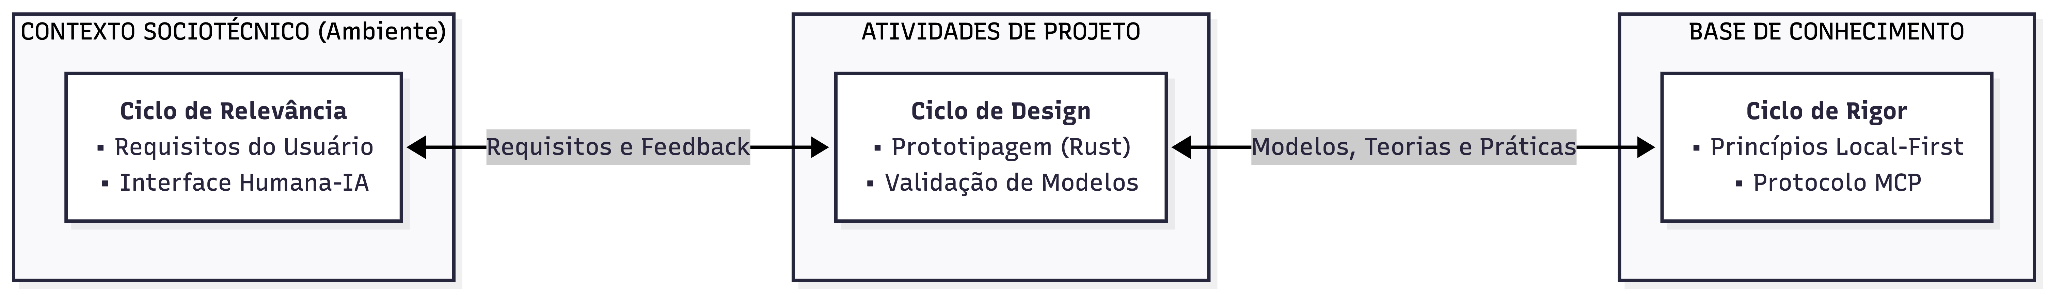
\includegraphics[width=\textwidth]{figuras/dsr-tres-ciclos.png}
\fonte{Elaboração própria.}
\end{figure}

No enquadramento FEDS (\textit{Framework for Evaluation in Design Science Research}) \cite{venable2016}, a avaliação disponível é \textit{artificial + somativa}: mede um artefato em cenário sintético e reporta seus resultados, sem observar uso ordinário. O estudo futuro de dois braços é \textit{naturalística + somativa}, pois observará tarefas pareadas em condições de uso definidas. A evidência artificial-somativa atual tem, portanto, teto de generalização: sustenta somente os controles e a latência interna nas condições instrumentadas.

\section{Procedimentos Metodológicos}
Seguindo a sistematização de Peffers et al. \cite{peffers2007}, a pesquisa executa seis atividades: (i) identificação do problema; (ii) definição de requisitos de localidade e uso de segredos; (iii) modelagem arquitetural e projeto dos componentes; (iv) demonstração integrada; (v) avaliação experimental de latência interna e cobertura de controles; e (vi) comunicação técnico-científica dos resultados. O traço de Peffers é parcialmente retrospectivo, pois o artefato antecedeu esta proposição. Há, contudo, evidência documentada de iteração construir--avaliar: ADRs registram a correção do \textit{gate} de consentimento para o modo NATIVE e as sondas A9/A10 subsequentes, constituindo um artefato genuíno do ciclo de rigor e \textit{design}. A avaliação de nuvem e de decisão humana é explicitamente futura.

\section{Artefatos Produzidos}
De acordo com a taxonomia de March e Smith \cite{march1995}, a pesquisa propõe e entrega:
\begin{itemize}
\item \textbf{Modelo}: arquitetura de referência para mediação de acessos a dados locais;
\item \textbf{Método}: protocolo de mediação, controle de escopo, consentimento e higienização de saída em tempo de execução;
\item \textbf{Instanciação}: protótipo \textit{Sovereign Vault}, operando sobre credenciais e segredos locais como representação empírica da proposta.
\end{itemize}
Não se afirma que a instância entregue seja um sistema RAG ou um repositório de contexto geral: suas operações avaliadas são leituras nomeadas por \textit{contêiner} e arquivo.

\section{Arquitetura de Referência Proposta}
A arquitetura separa logicamente o processamento cognitivo remoto dos repositórios privados da borda; essa separação não equivale a isolamento de processo ou de sistema operacional. Na Figura~\ref{fig:arquitetura-referencia} são representados os quatro módulos e a fronteira de confiança local. O agente externo permanece fora dessa fronteira, e a separação indicada é somente lógica. O sistema estrutura-se em módulos, detalhados nas próximas sub-seções.

\begin{figure}[htbp]
\centering
\caption{Arquitetura de referência da instância Sovereign Vault.}
\label{fig:arquitetura-referencia}
\resizebox{\textwidth}{!}{%
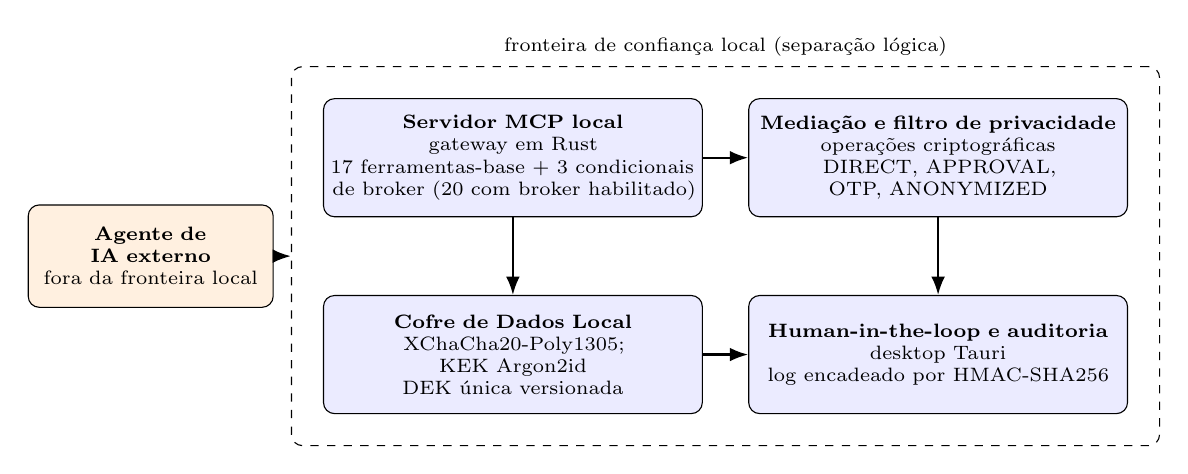
\begin{tikzpicture}[font=\scriptsize, >=Latex,
  module/.style={draw, rounded corners, align=center, text width=4.6cm, minimum height=1.5cm, fill=blue!8, inner sep=3pt},
  ext/.style={draw, rounded corners, align=center, text width=2.9cm, minimum height=1.3cm, fill=orange!12, inner sep=3pt},
  arr/.style={->, thick}]
  \node[module] (mcp)   at (0,0)      {\textbf{Servidor MCP local}\\gateway em Rust\\17 ferramentas-base + 3 condicionais\\de broker (20 com broker habilitado)};
  \node[module] (med)   at (5.4,0)    {\textbf{Mediação e filtro de privacidade}\\operações criptográficas\\DIRECT, APPROVAL, OTP, ANONYMIZED};
  \node[module] (vault) at (0,-2.5)   {\textbf{Cofre de Dados Local}\\XChaCha20-Poly1305; KEK Argon2id\\DEK única versionada};
  \node[module] (audit) at (5.4,-2.5) {\textbf{Human-in-the-loop e auditoria}\\desktop Tauri\\log encadeado por HMAC-SHA256};
  \node[draw, dashed, rounded corners, fit=(mcp)(med)(vault)(audit), inner sep=0.40cm,
        label={[font=\scriptsize]above:fronteira de confiança local (separação lógica)}] (boundary) {};
  \node[ext] (agent) at (-4.6,-1.25) {\textbf{Agente de IA externo}\\fora da fronteira local};
  \draw[arr] (agent.east) -- (boundary.west);
  \draw[arr] (mcp) -- (med);
  \draw[arr] (mcp) -- (vault);
  \draw[arr] (med) -- (audit);
  \draw[arr] (vault) -- (audit);
\end{tikzpicture}}
\fonte{Elaboração própria.}
\end{figure}

\subsection{Cofre de Dados Local}
O \textit{Sovereign Vault} armazena conteúdo localmente cifrado com XChaCha20-Poly1305. A custódia usa frase-secreta, da qual se deriva uma chave de cifragem de chaves (\textit{Key Encryption Key} -- KEK) via Argon2id, ou chaveiro do sistema operacional, que mantém a KEK no modo correspondente. A chave de cifragem de dados (\textit{Data Encryption Key} -- DEK) versionada é envolvida pela KEK em \codigo{keyring.svault}; há uma única DEK ativa, sem chaves por contêiner (\codigo{crates/sv-core/src/lib.rs:372-447,485-515}; \codigo{crates/sv-core/src/keyring.rs:206-282}; \codigo{crates/sv-crypto/src/lib.rs:92-103,149-193}). Nomes lógicos, modos, tamanhos de \textit{blobs} e outros metadados podem permanecer visíveis.

\subsection{Servidor MCP Local}
O \textit{gateway}, desenvolvido em Rust, expõe e gerencia ferramentas locais, interceptando requisições de agentes de IA. A superfície MCP analisada contém 17 ferramentas-base e três ferramentas condicionais de \textit{broker}, totalizando 20 quando o \textit{broker} está habilitado (\codigo{crates/sv-mcp/src/lib.rs:2370-2380,2461-2699}).

\subsection{Mediação, Filtro de Privacidade e Operações Criptográficas}
Os modos de \textit{contêiner} efetivamente suportados no \textit{desktop} são DIRECT, APPROVAL, OTP (senha de uso único, do inglês \textit{One-Time Password}) e ANONYMIZED. Leituras de arquivos em \textit{contêineres} DIRECT dispensam confirmação, enquanto operações de gestão de \textit{contêineres} seguem regras próprias de aprovação; APPROVAL e OTP passam pelo consentimento; ANONYMIZED mascara a saída de leituras UTF-8 sem solicitar aprovação. ZKP e NATIVE são valores de enumeração reservados e rejeitados, não mecanismos de isolamento avaliados (\codigo{apps/desktop/src-tauri/src/lib.rs:772-819}; \codigo{crates/sv-mcp/src/lib.rs:1431-1466}).

O mascaramento heurístico de saída de informação pessoal identificável (\textit{Personally Identifiable Information} -- PII) cobre exatamente e-mail, CPF, CNPJ, números de cartão válidos por Luhn, IPv4, telefones explicitamente formatados e SSN dos Estados Unidos (\codigo{crates/sv-privacy/src/lib.rs:49-64,206-233,483-575}). A versão avaliada não detecta RG, CEP, nomes completos, endereços, datas de nascimento ou telefones locais sem formatação. Por exemplo, \textit{João Silva, Rua X, CEP 12345-678} passa sem máscara. Como nomes completos, endereços, RG, CEP e telefones sem formatação passam sem máscara, um documento com CPF ou CNPJ mascarados, mas com nome e endereço expostos, pode permanecer identificável sob o Art.~5º da LGPD. O artefato não é adequado a documentos em que a vinculação de identidade por campos não mascarados seja risco realista; ele reduz exposição em saída textual, mas não é garantia genérica de anonimização ou de conformidade à LGPD.

Nas operações MCP documentadas, a semente privada e as chaves simétricas não são retornadas ao agente; somente assinatura, cifra ou texto decifrado são retornados após autorização (\codigo{crates/sv-core/src/transit.rs:245-330,368-392}; \codigo{crates/sv-mcp/src/lib.rs:1317-1422,1946-1972}). A zeroização ponta a ponta da semente Ed25519 depende também da disciplina de armazenamento do chamador em \codigo{sv-core}, e não apenas de \codigo{sv-crypto}. No \textit{desktop}, operações de trânsito e assinatura exigem aprovação por operação. Esta versão não fornece autorização vinculada à chave/uso nem apresenta ao usuário uma descrição verificável do conteúdo a assinar ou decifrar; portanto o resultado de protocolo não elimina risco de uso como oráculo.

\phantomsection\label{nota:headless}
\svnota{\textbf{Aviso de segurança -- modo \textit{headless}.} Durante o ciclo de rigor DSR, a revisão de código identificou apagamento de escopos e um oráculo \textit{modeless} de criptografia/corretagem. A correção aplicada preserva os escopos persistidos do agente ao autenticá-lo e recusa, em modo \textit{headless}, operações \textit{modeless} que portam ou usam segredos (cifra de trânsito, decifragem, assinatura e corretagem), de forma \textit{fail-closed}; essas operações devem usar o aplicativo \textit{desktop} (\codigo{apps/cli/src/serve.rs}). Assim, o \textit{headless} mantém operações de \textit{contêiner} em modo DIRECT (criação, destruição, leitura, escrita e remoção de arquivos) e consultas de metadados (listagem de \textit{contêineres} e arquivos, \codigo{vault.info}, verificação de auditoria e listagem de chaves de trânsito e assinatura, que retornam nome, versão e chave pública, nunca bytes secretos), mas não oferece consentimento humano para operações secretas.}

\subsection{\textit{Human-in-the-loop} e Auditoria}
A interface \textit{desktop} foi implementada em Tauri com política de segurança de conteúdo (\textit{Content Security Policy} -- CSP) e capacidades explícitas (\codigo{apps/desktop/src-tauri/tauri.conf.json:24-26}; \codigo{apps/desktop/src-tauri/capabilities/default.json:1-9}). O presente estudo não mede comparativamente superfície de injeção, isolamento de segurança ou consumo de memória em relação ao Electron.

Operações sensíveis geram registros encadeados por código de autenticação de mensagem baseado em resumo criptográfico (\textit{Hash-based Message Authentication Code} -- HMAC) com SHA-256, verificados contra \textit{checkpoint} autenticado local (\codigo{crates/sv-audit/src/lib.rs:545-727,977-1056}). Isso fornece evidência de adulteração, remoção e truncamento em relação ao \textit{checkpoint} presente. Não é prova de armazenamento \textit{append-only} resistente a \textit{rollback}: uma restauração completa e internamente consistente do diretório de auditoria não é detectável sem âncora externa confiável, como \textit{log} de transparência remoto ou contador monotônico protegido.

\section{Modelo de Execução e Protocolo de Segurança}
No caminho \textit{desktop WebSocket} autenticado, o fluxo de solicitações passa por autenticação, validação de parâmetros e caminhos, verificação de escopo, política de consentimento quando aplicável, operação no cofre, filtragem ANONYMIZED quando aplicável e auditoria. Na Figura~\ref{fig:fluxo-requisicao} é explicitada a ordem desses estágios e os dois pontos condicionais. Leituras em \textit{contêineres} DIRECT retornam dados sem consentimento por projeto; por isso, \textit{contêineres} DIRECT ficam fora da garantia de mediação humana. Trata-se de uma relação de compromisso deliberada que o usuário deve configurar conscientemente. Nas operações criptográficas, o \textit{gateway} executa localmente a operação e retorna a saída do protocolo, e não \textit{bytes} de chave; a limitação de oráculo e de transparência de consentimento descrita acima permanece aplicável.

\begin{figure}[htbp]
\centering
\caption{Fluxo de execução de uma requisição no caminho desktop WebSocket autenticado.}
\label{fig:fluxo-requisicao}
\resizebox{\textwidth}{!}{%
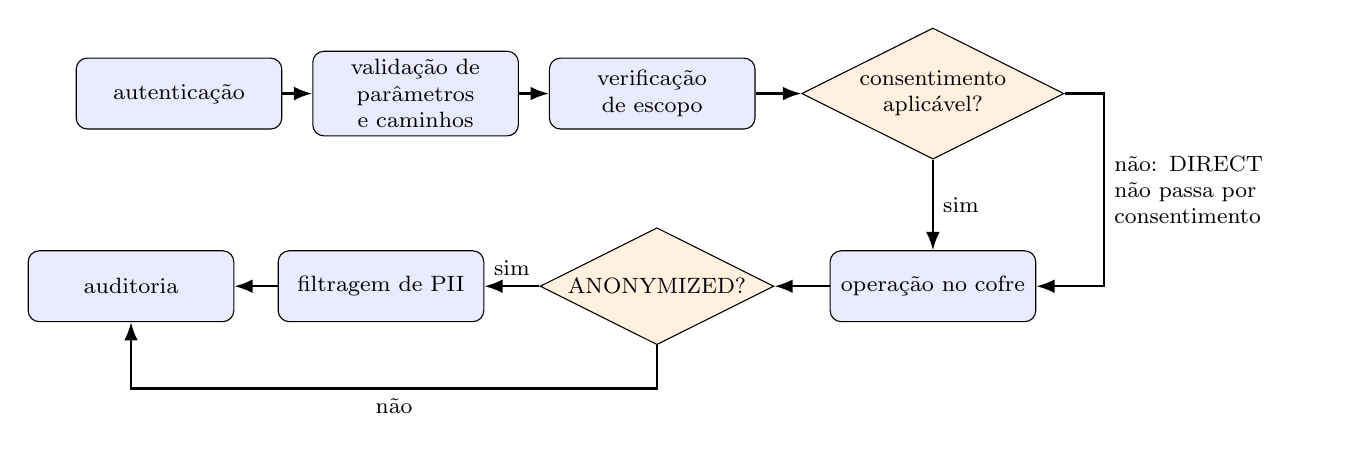
\begin{tikzpicture}[font=\footnotesize, >=Latex,
  etapa/.style={draw, rounded corners, align=center, text width=2.4cm, minimum height=0.9cm, fill=blue!8, inner sep=3pt},
  decision/.style={draw, diamond, aspect=2.0, align=center, inner sep=1.5pt, fill=orange!12},
  arr/.style={->, thick}]
  \node[etapa] (auth) {autenticação};
  \node[etapa, right=0.38cm of auth] (valid) {validação de\\parâmetros e caminhos};
  \node[etapa, right=0.38cm of valid] (scope) {verificação de escopo};
  \node[decision, right=0.58cm of scope] (cons) {consentimento\\aplicável?};
  \node[etapa, below=1.15cm of cons] (vaultop) {operação no cofre};
  \node[decision, left=0.70cm of vaultop] (anon) {ANONYMIZED?};
  \node[etapa, left=0.70cm of anon] (filter) {filtragem de PII};
  \node[etapa, left=0.55cm of filter] (auditflow) {auditoria};
  \draw[arr] (auth) -- (valid);
  \draw[arr] (valid) -- (scope);
  \draw[arr] (scope) -- (cons);
  \draw[arr] (cons) -- node[right, font=\footnotesize] {sim} (vaultop);
  \draw[arr] (cons.east) -- ++(0.5,0) |- node[pos=.25, right, font=\footnotesize, align=left, text width=2.5cm] {não: DIRECT\\não passa por\\consentimento} (vaultop.east);
  \draw[arr] (vaultop) -- (anon);
  \draw[arr] (anon) -- node[above, font=\footnotesize] {sim} (filter);
  \draw[arr] (anon.south) -- ++(0,-0.55) -| node[pos=.25, below, font=\footnotesize] {não} (auditflow.south);
  \draw[arr] (filter) -- (auditflow);
\end{tikzpicture}}
\fonte{Elaboração própria.}
\end{figure}

\svnota{\textbf{Modelo de ameaça e limites.} O estudo avalia um usuário, uma máquina e um \textit{gateway} local desbloqueado. O adversário principal é um agente MCP autenticado e potencialmente comprometido. Estão fora de escopo: comprometimento do sistema operacional, \textit{malware} ou processo sob a mesma conta do usuário, inspeção de memória, vulnerabilidades em dependências nativas/TCB, retenção de dados pelo provedor de IA e \textit{rollback} completo da auditoria. Roubo de \textit{token} também está fora de escopo: o \textit{token} está em claro no ambiente do cliente; como trabalho futuro, recomenda-se arquivo com permissão 0600 ou chaveiro do sistema operacional. Atacante adaptativo está fora de escopo da bateria de execução única; teste adaptativo é trabalho futuro. Leituras DIRECT retornam dados sem consentimento por projeto, e contêineres DIRECT estão fora da garantia de mediação humana; essa relação de compromisso deve ser configurada conscientemente pelo usuário. A confidencialidade em repouso protege conteúdo cifrado, mas nomes e metadados operacionais podem permanecer visíveis. O modo \textit{headless} preserva escopos e bloqueia operações secretas \textit{modeless}; os resultados experimentais de menor privilégio e mediação humana, porém, referem-se ao \textit{gateway desktop WebSocket}.}

\section{Estratégia de Desenvolvimento do Artefato}
O protótipo é codificado em Rust. A proibição de \codigo{unsafe} nos \textit{crates} próprios reduz classes de erros de corrupção de memória no código de aplicação auditado (por exemplo, \codigo{crates/sv-mcp/src/lib.rs:18}). Não se infere daí ausência de vulnerabilidades críticas, isolamento de memória no SO ou redução mensurada de latência. Tauri foi escolhido para a interface com CSP e capacidades explícitas, sem alegação comparativa perante Electron.

\section{Dados da Avaliação}
\label{sec:dados-avaliacao}
Os dados da avaliação são gerados sinteticamente pelo \textit{harness} \codigo{apps/thesis-eval}: ele cria um cofre temporário, semeia arquivos e dirige o \textit{gateway} real. Portanto, os dados não provêm de repositório externo. O uso de dados pessoais reais para medir o filtro de PII criaria o próprio risco que o artefato busca mitigar; por não haver necessidade para a medição, não se trata dado pessoal real, em consonância com a minimização esperada pela LGPD.

Em \codigo{payload_for}, nas linhas 466--478 de \codigo{apps/thesis-eval/src/main.rs}, as condições não ANONYMIZED usam um preenchimento sem PII, e a condição ANONYMIZED usa, para que o filtro execute trabalho sobre conteúdo marcado, uma unidade portadora de PII. As duas unidades são, respectivamente:
\begingroup
\footnotesize
\begin{verbatim}
lorem ipsum dolor sit amet consectetur adipiscing elit;
user jane.doe@example.com cpf 529.982.247-25 ip 192.168.0.1;
\end{verbatim}
\endgroup
As unidades são repetidas e truncadas exatamente em 128 B, 1 KiB (1.024 B) e 16 KiB (16.384 B), com N=1.000 requisições por célula. Os identificadores são fictícios ou pertencem a faixas reservadas: \codigo{example.com} é reservado para documentação pelo documento normativo \textit{Request for Comments} (RFC) 2606 \cite{rfc2606}, \codigo{192.168.0.1} pertence ao espaço IPv4 privado definido na RFC 1918 \cite{rfc1918}, e o CPF apresentado é um número de teste amplamente usado, válido somente no dígito verificador e não atribuído a pessoa real.

As cargas ANONYMIZED contêm exatamente três das sete categorias detectadas pelo filtro: e-mail, CPF e IPv4. Assim, o custo observado para o filtro é específico dessa composição e não corresponde a uma média sobre documentos reais. O subcomando \codigo{micro} usa a mesma unidade de PII em \codigo{pii_payload}, linhas 315--323, o que torna o custo isolado comparável ao estágio $T_{filter}$ do gateway.

A bateria adversarial contém 12 sondas pré-especificadas no código: A1--A10 são ataques e C1--C2 são controles. O \textit{harness} materializa \codigo{target/thesis-eval/adversarial.csv} com os campos \codigo{id}, \codigo{class}, \codigo{blocked}, \codigo{transport_error}, \codigo{expected_block}, \codigo{pass} e \codigo{description}; o veredito esperado é declarado antes da execução, o que evita seleção \textit{post-hoc} de resultados.

O campo \codigo{transport_error} separa decisão de política de ruído de infraestrutura. Uma sonda cuja troca não alcança veredito do servidor -- falha de conexão, de envio ou de leitura do fluxo -- não informa nada sobre o controle avaliado; contá-la como bloqueio faria um soquete instável parecer defesa em funcionamento. Essas observações são, portanto, excluídas do numerador \textbf{e} do denominador da taxa de bloqueio e da taxa de disponibilidade, e reportadas à parte pelo agregador (\codigo{docs/thesis/evidence/aggregate.py}). A rejeição de pareamento não é falha de transporte: o servidor respondeu e recusou as credenciais, de modo que permanece classificada como bloqueio. O CSV da execução preliminar reproduzido no Apêndice~\ref{cap:reprodutibilidade} antecede a introdução dessa coluna e é lido como se nenhuma sonda tivesse falhado em transporte, o que corresponde ao ocorrido naquela execução.

A Tabela~\ref{tab:dados-avaliacao} resume a composição do conjunto sintético descrito nesta seção. As medições por chamada do \textit{gateway} são coletadas por \codigo{TimingSink} nos estágios \codigo{validate}, \codigo{authorize}, \codigo{execute} e \codigo{filter}, e são agregadas em média, p50 e p95 em \codigo{latency.csv}. O subcomando \codigo{micro} materializa as medições isoladas em \codigo{micro.csv}, e a bateria materializa os vereditos pré-especificados em \codigo{adversarial.csv}. A execução preliminar desses três arquivos contém uma sessão e não apresenta intervalo de confiança (IC); a reavaliação de latência em \codigo{docs/thesis/evidence/v2/} contém dez sessões com IC de 95\% por \textit{bootstrap}; a execução definitiva requer $k\geq3$ sessões e IC de 95\% por \textit{bootstrap}, como especificado no plano de avaliação.

\begin{table}[htbp]
\centering
\caption{Conjunto sintético da avaliação atual.}
\label{tab:dados-avaliacao}
\begin{tabularx}{\textwidth}{>{\bfseries}p{0.24\textwidth}X}
\toprule Elemento & Característica \\ \midrule
Condições & DIRECT, APPROVAL--AutoAllow, OTP--AutoAllow e ANONYMIZED \\
Cargas & 128 B, 1 KiB e 16 KiB, geradas e truncadas sinteticamente \\
Repetições & N=1.000 requisições por célula \\
Medido & estágios do gateway e vereditos das 12 sondas pré-especificadas \\
\bottomrule
\end{tabularx}
\fonte{Elaboração própria a partir de \codigo{apps/thesis-eval/src/main.rs}. Para o protocolo do \textit{microbenchmark}, ver Tabela~\ref{tab:metodologia-microbenchmark}.}
\end{table}

\section{Plano de Avaliação}
A validação utiliza metodologias de avaliação naturalísticas e artificiais \cite{venable2016}. No FEDS, a evidência atual é artificial + somativa; o protocolo futuro de dois braços será naturalística + somativa. A evidência atualmente disponível é de uma leitura sintética pelo \textit{gateway} local e de uma bateria finita de solicitações; por isso o plano separa variáveis observáveis no \textit{gateway} de variáveis de usuário, rede e nuvem, com generalização limitada às condições artificiais instrumentadas.

\subsection{Avaliação de Latência}
O desenho do \textit{microbenchmark} filia-se à tradição de avaliação de desempenho por variável de resposta, fatores e níveis, aplicada por Silva et al. \cite{silva2016} à medição de algoritmos criptográficos em sistema embarcado e em computador de propósito geral: o estimando é definido antes da coleta, os fatores controlados são o modo de \textit{contêiner} e o tamanho da carga, em desenho fatorial completo de quatro modos por três cargas, e o custo é reportado por operação, com média e percentis. Para uma leitura local mediada, define-se:
\begin{equation}
\resizebox{\textwidth}{!}{$\displaystyle T_{gateway}=T_{parse+validacao+escopo}+T_{cofre}+I_{anon}(T_{mascaramento})+I_{consentimento}(T_{espera\ humana}+T_{despacho})$}
\label{eq:gateway}
\end{equation}
Na Equação~\eqref{eq:gateway}, o indicador $I$ vale 1 somente quando o modo correspondente é aplicado. No \textit{microbenchmark stdio} atual, o termo $T_{parse+validacao+escopo}$ observa somente validação de parâmetros e caminho: o transporte usa \codigo{PairState::AlreadyPaired(None)}, portanto não há resolução de agente nem aplicação de escopo nesse caminho. O custo de \codigo{enforce_scopes} não é medido neste \textit{microbenchmark}; ele é medido separadamente no transporte \textit{WebSocket} autenticado (Seção~\ref{sec:custo-escopos}). Para uma única chamada MCP instrumentada, define-se separadamente:
\begin{equation}
T_{e2e}^{(1)}=T_{cliente,\,serializacao}+T_{transporte,\,ida}+T_{gateway}+T_{transporte,\,volta}+T_{cliente,\,recebimento}.
\label{eq:e2e}
\end{equation}
O estimando $T_{e2e}^{(1)}$ da Equação~\eqref{eq:e2e} começa imediatamente antes da serialização em JSON-RPC (\textit{JavaScript Object Notation Remote Procedure Call}) no cliente e termina quando o cliente recebe a resposta completa; ida e volta do transporte são termos disjuntos. Ele exclui planejamento/inferência do modelo, filas externas, interação do usuário e múltiplas voltas ferramenta--modelo. Ainda não foi medido e não sustenta inferência sobre experiência do usuário até haver instrumentação desses \textit{timestamps}. Para APPROVAL e OTP, $T_{espera\ humana}$ deve ser relatado como distribuição (mediana, p95 e taxa de timeout/negação), e não como parcela em microssegundos.

\begin{table}[htbp]
\centering
\caption{Metodologia do \textit{microbenchmark} atual.}
\label{tab:metodologia-microbenchmark}
\begin{tabularx}{\textwidth}{>{\bfseries}p{0.29\textwidth}X}
\toprule Campo & Estado na evidência atual \\ \midrule
Unidade de análise & uma leitura sintética \codigo{vault.read} pelo gateway local em \textit{stdio} \\
Condições & DIRECT, APPROVAL--AutoAllow, OTP--AutoAllow e ANONYMIZED \\
Cargas & 128 B, 1 KiB e 16 KiB \\
N & na execução sob protocolo corrigido, $k=10$ sessões com $n=1.000$ requisições medidas por célula, 200 chamadas de aquecimento descartadas e ordem de células aleatorizada por sessão; estatística: mediana por célula com IC de 95\% por \textit{bootstrap} percentílico \\
Medido & validação de parâmetros/caminho (sem resolução de agente nem escopo no caminho \textit{stdio}), despacho do controlador, leitura local do cofre e filtro de PII \\
Não medido & custo de \codigo{enforce_scopes} no caminho \textit{stdio} (medido à parte no \textit{WebSocket}, Tabela~\ref{tab:enforce-scopes}), escrita de auditoria (excluída da soma de estágios; ver Seção~\ref{sec:fronteira-evidencia}), decisão humana, rede de longa distância (\textit{Wide Area Network} -- WAN), inferência em nuvem, carga de produção e utilidade de tarefa \\
\bottomrule
\end{tabularx}
\fonte{Elaboração própria a partir de \codigo{apps/thesis-eval/src/main.rs} e \codigo{target/thesis-eval/latency.csv}.}
\end{table}

\subsection{Avaliação da Preservação de Privacidade}
A avaliação de segurança utiliza uma bateria pré-especificada de chamadas JSON-RPC e controles legítimos, em uma execução de caixa-preta. Ela valida somente transporte \textit{WebSocket}, escopo, validação de caminho e aplicação de política de humano no circuito (\textit{Human-in-the-Loop} -- HITL) simulada (\codigo{HitlPolicy}); não exercita o controlador real de consentimento \textit{desktop} \codigo{ApprovalState}. Não estima taxa populacional de bloqueio de \textit{prompt injection}: as ``injeções'' são simuladas pelo efeito final (chamadas de ferramenta) e não por um LLM real submetido a conteúdo adversarial. A validade externa, portanto, restringe-se ao protocolo e às negativas enumeradas.

\subsection{Protocolo Futuro de Comparação em Nuvem}
Uma comparação com nuvem não foi executada. Como avaliação futura, o protocolo de dois braços em \codigo{docs/thesis/EVAL-PROTOCOL.md} compara \textit{Arm} A (mesmo modelo acessando dados somente pelo \textit{gateway} local) e \textit{Arm} B (mesmo modelo/versão recebendo o material sintético diretamente por um caminho de contexto em nuvem). A evidência corrente fornece apenas parte do \textit{Arm} A; adaptador de nuvem, telemetria, política de \textit{baseline}, governança e análise estatística ainda são necessários.

\section{Considerações Finais}
Este capítulo define o método DSR e a arquitetura \textit{Local-First} integrada ao MCP. O artefato permite estudar mediação de segredos e credenciais, mas não responde empiricamente por RAG, isolamento de processo/SO, consentimento humano mensurado ou comparação com nuvem. O capítulo seguinte apresenta somente os dados efetivamente produzidos pelo \textit{harness}.

\chapter{RESULTADOS}
\section{Considerações Iniciais}
Neste capítulo são apresentados os resultados obtidos com o artefato. A leitura começa pela fronteira de evidência, que fixa o que os dados sustentam e sob quais qualificações, e segue pelo \textit{microbenchmark} de leitura local mediada, pelo custo de imposição de escopos no caminho \textit{WebSocket}, pela bateria adversarial pré-especificada e pela síntese que responde às questões de pesquisa e confronta o resultado com os trabalhos correlatos.

\section{Fronteira de Evidência}
\label{sec:fronteira-evidencia}
Na Tabela~\ref{tab:fronteira-evidencia} é delimitado o que os dados e o código efetivamente sustentam e, para cada alegação, a qualificação que a acompanha obrigatoriamente. Ela funciona como contrato de leitura do restante do capítulo: nenhuma afirmação posterior deve ser interpretada além do que essa fronteira permite.

\begin{table}[htbp]
\centering
\small
\caption{O que os dados e o código sustentam, e suas qualificações.}
\label{tab:fronteira-evidencia}
\begin{tabularx}{\textwidth}{>{\raggedright\arraybackslash}p{0.23\textwidth}>{\raggedright\arraybackslash}p{0.36\textwidth}X}
\toprule Alegação & Evidência reportável & Qualificação obrigatória \\ \midrule
Armazenamento local cifrado & XChaCha20-Poly1305, KEK Argon2id e DEK & sem chaves por \textit{contêiner}; metadados visíveis \\
Mediação MCP \textit{desktop} & implementação \textit{desktop WS} de escopos, APPROVAL/OTP e auditoria & o resultado 10/10 usa \codigo{HitlPolicy} simulada e não exercita o controlador real de consentimento \textit{desktop}; \textit{headless} excluído \\
Sem retorno de bytes de chave & implementação de trânsito/assinatura & não elimina abuso como oráculo \\
Redução de PII & sete categorias heurísticas em saída ANONYMIZED; \textit{recall} canônico 100\% (200/200 por categoria) e 0\% de falso positivo (0/500 por categoria) em identificadores sintéticos & não é anonimização genérica/LGPD; somente texto; robustez a formato varia por categoria (Tabela~\ref{tab:pii-robustez}); NÃO detecta RG, CEP, nomes, endereços, datas de nascimento e telefones sem formatação \\
Sobrecarga local & \textit{microbenchmark} sob protocolo corrigido: $k=10$ sessões, $n=1.000$ por célula, mediana com IC de 95\% por \textit{bootstrap} & sem humano, WAN, inferência, baseline de nuvem ou utilidade; o total soma estágios e exclui a escrita de auditoria \\
Custo de escopos & \codigo{enforce_scopes} no caminho \textit{WebSocket}: entre 2,1 e 2,2\micro{} com 20 escopos, IC excluindo zero nas três cargas & braços de escopo em ordem fixa por sessão; célula de 1 escopo/128 B com delta negativo implausível (Tabela~\ref{tab:enforce-scopes}) \\
Resultado adversarial & bateria original: 10/10 sondas e 2/2 controles, sem falhas de transporte; extensão a 24 sondas: 11/12 vereditos pré-especificados confirmados e cobertura 17/20 & valida transporte WS, escopo, caminho e política simulada; A11--A15 dirigem o binário real como subprocesso; sem atacante adaptativo ou inferência de taxa populacional \\
\bottomrule
\end{tabularx}
\fonte{Elaboração própria com base nos \textit{crates} citados e nos artefatos em \codigo{target/thesis-eval} e \codigo{docs/thesis/evidence/v2}.}
\end{table}

Uma limitação de instrumentação aplica-se a todas as tabelas de latência deste capítulo. O total reportado por \codigo{StageTimings} é a soma dos estágios \codigo{validate}, \codigo{authorize}, \codigo{execute} e \codigo{filter}, e não um relógio de parede: a escrita obrigatória de auditoria pré-execução ocorre entre \codigo{authorize} e \codigo{execute} e, portanto, nunca é contada. Como a auditoria com evidência de adulteração é um dos pilares da arquitetura, seu custo é invisível em toda a avaliação de desempenho aqui reportada: a sobrecarga de mediação medida exclui o custo da escrita de auditoria. Esse custo não foi medido, e não é estimado aqui; sua instrumentação, como um quinto estágio de \codigo{StageTimings}, consta dos trabalhos futuros.

\section{Microbenchmark Sintético de Leitura Local Mediada}
O \textit{microbenchmark} cria cofre temporário, semeia cargas sintéticas e executa leituras reais pelo \textit{gateway} local. A execução preliminar de uma sessão, publicada em versão anterior deste texto, reportava DIRECT mais lento que APPROVAL--\textit{AutoAllow} e OTP--\textit{AutoAllow} nas seis comparações de média por carga. DIRECT executa um subconjunto estrito do trabalho desses dois modos, o que torna essa ordenação inesperada sob o modelo simples de trabalho adicional; os resultados disponíveis não identificam sua causa. A reavaliação sobre este repositório mostrou que aquela tabela não é reprodutível: o \textit{harness} foi modificado após a coleta (227 inserções e 38 remoções em \codigo{apps/thesis-eval/src/main.rs}, \textit{commit} \codigo{2fb252b}), não existe \codigo{run-metadata.json} daquela execução, e o braço que replica seu protocolo recupera a inversão em apenas 2 dos 6 contrastes por mediana, nunca em 6/6. Os números daquela tabela são, portanto, retirados deste texto e substituídos pela Tabela~\ref{tab:latencia-pareada-v2}, obtida sob protocolo corrigido.

\begin{table}[htb]
\centering
\caption{Diferenças pareadas de latência entre DIRECT e os modos de consentimento sob o protocolo corrigido (ordem de célula aleatorizada por sessão, 200 chamadas de aquecimento descartadas por célula, $k=10$ sessões, $n=1000$ chamadas medidas por célula). Estatística: média das diferenças pareadas entre medianas por sessão, com IC95\% \textit{bootstrap} percentílico ($B=10\,000$, reamostragem por sessão).}
\label{tab:latencia-pareada-v2}
\begin{tabular}{@{}llrrc@{}}
\toprule
Carga & Contraste & \shortstack[r]{Média de\\$\Delta$ p50 (\micro)} & IC95\% (\micro) & \shortstack[c]{Exclui\\zero?} \\
\midrule
128 B  & DIRECT $-$ APPROVAL & $+0{,}060$ & $[-0{,}046;\ 0{,}160]$ & Não \\
128 B  & DIRECT $-$ OTP      & $+0{,}046$ & $[-0{,}046;\ 0{,}136]$ & Não \\
1 KiB  & DIRECT $-$ APPROVAL & $-0{,}009$ & $[-0{,}106;\ 0{,}082]$ & Não \\
1 KiB  & DIRECT $-$ OTP      & $+0{,}009$ & $[-0{,}050;\ 0{,}084]$ & Não \\
16 KiB & DIRECT $-$ APPROVAL & $-0{,}134$ & $[-0{,}407;\ 0{,}063]$ & Não \\
16 KiB & DIRECT $-$ OTP      & $-0{,}032$ & $[-0{,}090;\ 0{,}023]$ & Não \\
\bottomrule
\end{tabular}
\fonte{\codigo{docs/thesis/evidence/v2/latency_v2_paired_diffs.csv}.}
\end{table}

Três resultados organizam a leitura da Tabela~\ref{tab:latencia-pareada-v2}. O primeiro é positivo e central para a QP2: nenhum dos seis IC de 95\% do contraste entre medianas exclui zero sob \textit{AutoAllow}, sem que isso constitua teste de equivalência. O experimento não distingue de zero o custo de APPROVAL e OTP sobre DIRECT, e o desenho não mede a espera humana. Em produção, $T_{espera\ humana}$ permanece dominado pelo tempo de reação humana, tipicamente em segundos, parâmetro externo não medido pelo \textit{gateway}.

O segundo resultado é a retirada da ordenação publicada: ela era um artefato de medição de origem não determinada. A lacuna de proveniência descrita acima, reescrita do \textit{harness} após a coleta, ausência de metadados de execução e não replicação a partir deste repositório, impede atribuir causa; o que os dados novos sustentam é somente que o padrão publicado não se reproduz a partir deste repositório.

A comparação entre estimandos evidencia sensibilidade à cauda da distribuição. Em 16 KiB, a diferença DIRECT$-$OTP calculada a partir das médias por sessão é $+6{,}005$\micro{}, com IC95\% $[5{,}690;\ 6{,}331]$, enquanto a média das diferenças entre medianas por sessão é $-0{,}032$\micro{}, com IC95\% $[-0{,}090;\ 0{,}023]$. O p99 de DIRECT varia entre 38,5 e 61,7\micro{} entre sessões, contra mediana próxima de 29\micro{}. Esses resultados descrevem aspectos distintos da distribuição: o contraste baseado em medianas é o estimando adotado para a latência central, mas não invalida o resultado baseado em médias nem demonstra ausência de efeito na cauda.

\svnota{\textbf{Nota metodológica sobre a tabela retirada.} A tabela preliminar apresenta seis diferenças de mesmo sinal, mas os contrastes compartilham condições e uma única sessão. Os resumos disponíveis não permitem estabelecer independência entre esses contrastes nem reconstruir a variância necessária para quantificar sua distância de zero em erros-padrão. Por isso, o padrão é tratado como observação descritiva, sem atribuição de causa sistemática. A ausência de metadados e a modificação posterior do \textit{harness} limitam a reprodutibilidade da execução original.}

Para delimitar a origem provável do artefato, uma ablação $2\times2$ variou a ordem de execução das células e o descarte de aquecimento (Tabela~\ref{tab:ablacao-ordem} e Figura~\ref{fig:ablacao-ordem}). A fração de contrastes com sinal invertido cai de 70,0--73,3\% nos braços de ordem fixa para 53,3--56,7\% nos braços de ordem aleatorizada.

\begin{table}[htb]
\centering
\caption{Ablação $2\times2$ de ordem de execução e descarte de aquecimento ($k=5$ sessões por braço, $n=1000$). A fração de sinal invertido conta contrastes em que DIRECT mede mais lento que um superconjunto estrito do seu próprio trabalho, ordenação inesperada sob o modelo simples de trabalho adicional, cuja causa os resultados disponíveis não identificam.}
\label{tab:ablacao-ordem}
\begin{tabular}{clcrr}
\toprule
Braço & Ordem & Aquecimento & Sinal invertido & Efeito de posição \\
\midrule
A & fixa (protocolo publicado) & nenhum      & 70{,}0\% & $+0{,}029$\%/pos.$^{\dagger}$ \\
B & fixa            & descartado  & 73{,}3\% & $-0{,}015$\%/pos.$^{\dagger}$ \\
C & aleatorizada    & nenhum      & 53{,}3\% & $-0{,}174$\%/pos. \\
D & aleatorizada    & descartado  & 56{,}7\% & $-0{,}033$\%/pos. \\
\bottomrule
\end{tabular}

\vspace{2pt}
\footnotesize
$^{\dagger}$ Sob ordem fixa cada célula ocupa uma única posição em todas as sessões, de modo que célula e posição são colineares e a inclinação normalizada não é identificável. Os valores dos \textit{ARM} A e B não devem ser lidos como ausência de efeito de posição.

\fonte{\codigo{docs/thesis/evidence/v2/order_ablation_contrast_ci.csv}.}
\end{table}

\begin{figure}[htbp]
\centering
\caption[Ablação de ordem e aquecimento]{Ablação $2\times2$ de ordem de execução e aquecimento: fração de contrastes com sinal invertido por \textit{ARM} (painel esquerdo) e inclinação do efeito de posição-na-execução (painel direito). $k=5$ sessões por \textit{ARM}, $n=1000$. Sob ordem fixa (\textit{ARM} A e B), célula e posição são colineares e a inclinação normalizada não é identificável; os valores desses dois braços não devem ser lidos como estimativa do efeito de posição.}
\label{fig:ablacao-ordem}
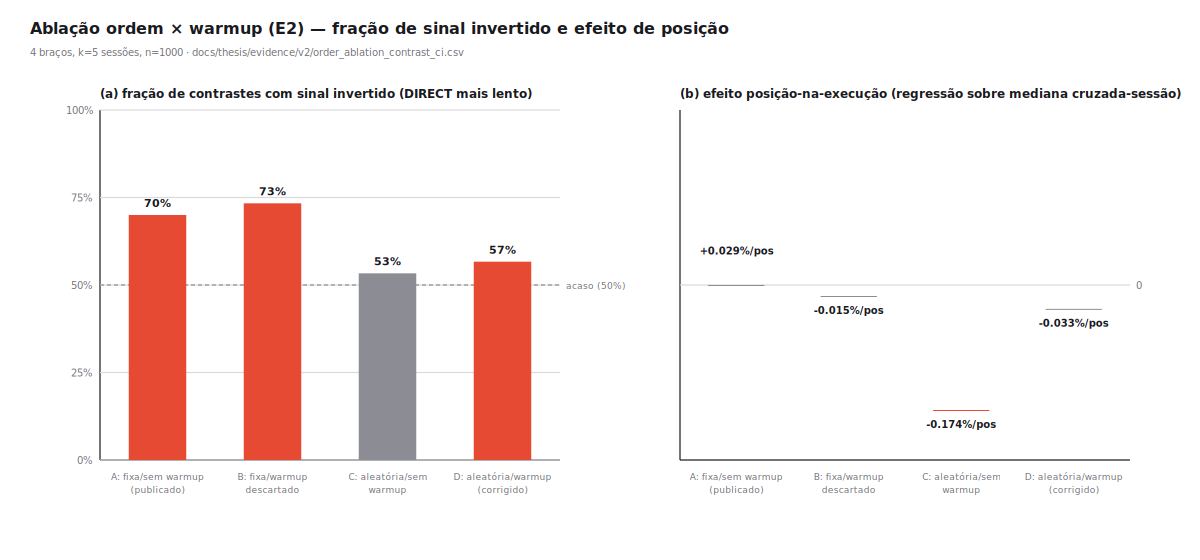
\includegraphics[width=\textwidth]{figuras/ablacao_ordem.png}
\fonte{Elaboração própria a partir de \codigo{docs/thesis/evidence/v2/order_ablation_contrast_ci.csv}.}
\end{figure}

Uma atribuição linear do tipo ``a posição na execução explica parte da inversão'' não é testável sob ordem fixa: cada célula ocupa exatamente uma posição em todas as sessões, célula e posição são perfeitamente colineares, e a inclinação normalizada por célula não é identificável, inclinação $\approx 0$ nos \textit{ARM} A e B é uma propriedade algébrica do estimador, não evidência de ausência de efeito. O padrão observado, inversão concentrada em 128 B e ausente nas cargas maiores, favorece um efeito categórico de estado frio sobre a primeira célula executada, em vez de uma deriva contínua por posição. A nota da Tabela~\ref{tab:ablacao-ordem} registra a ressalva de identificabilidade.

Na Figura~\ref{fig:latencia-estagios} são apresentadas as latências sob o protocolo corrigido. No painel esquerdo, o total p50 por carga é mostrado em escala log-log, com recorte linear de 0 a 40\micro{} para as menores cargas. No painel direito, são mostradas as diferenças pareadas DIRECT$-$APPROVAL/OTP com IC95\%, todos contendo zero. A figura mostra o aumento do total na condição ANONYMIZED; a atribuição desse aumento à filtragem depende da instrumentação e das medições de componentes, não de uma decomposição gráfica de estágios neste painel.

\begin{figure}[htbp]
\centering
\caption[Latência sob o protocolo corrigido]{Latência de leitura mediada sob o protocolo corrigido. Estimador: mediana (p50) por célula; $k=10$ sessões, $n=1000$ chamadas medidas por célula, 200 chamadas de aquecimento descartadas e ordem de células aleatorizada por sessão; IC de 95\% por \textit{bootstrap} percentílico ($B=10\,000$, reamostragem por sessão). Painel esquerdo: total por carga em escala log-log, com recorte linear de 0 a 40\micro{}; painel direito: diferenças pareadas DIRECT$-$APPROVAL/OTP com IC95\%, todos contendo zero.}
\label{fig:latencia-estagios}
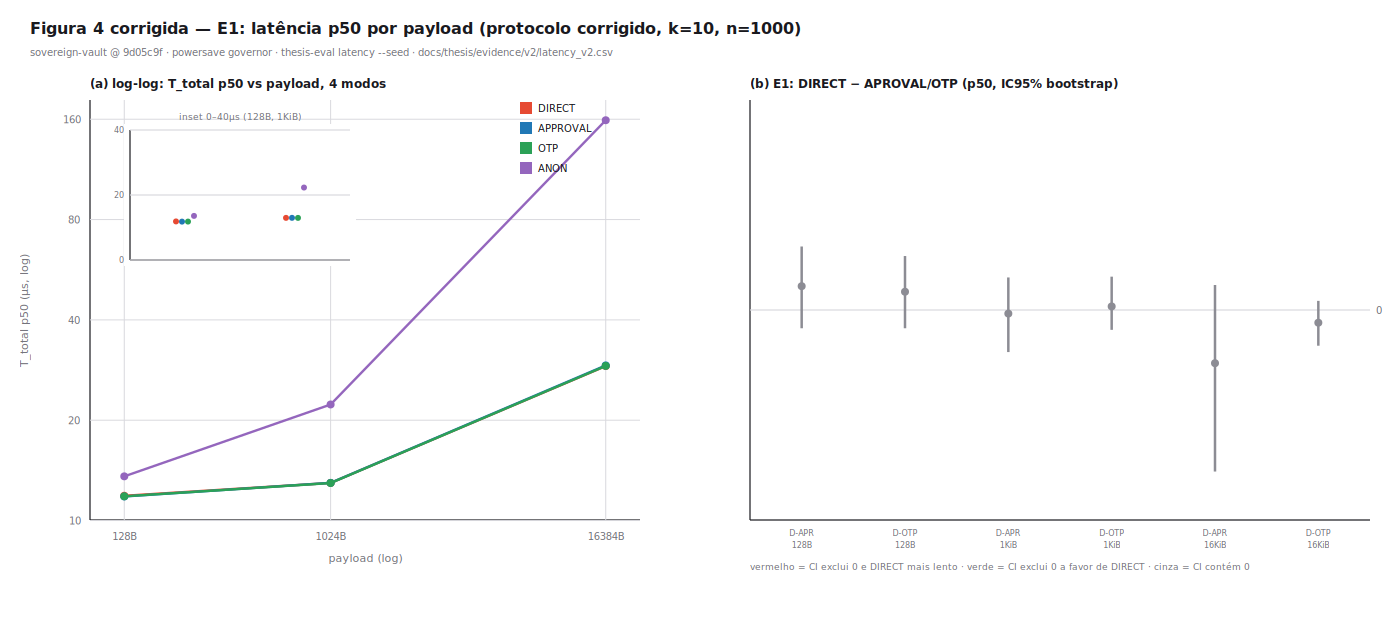
\includegraphics[width=\textwidth]{figuras/figura4_corrigida.png}
\fonte{Elaboração própria a partir de \codigo{docs/thesis/evidence/v2/latency_v2.csv}.}
\end{figure}

Medições isoladas dos componentes também estão disponíveis no arquivo \codigo{micro.csv} do mesmo diretório de avaliação, na execução preliminar de uma sessão e sem intervalo de confiança: para 128 B, 1 KiB e 16 KiB, a leitura/decifra teve médias de 4,14\micro{}, 4,97\micro{} e 16,82\micro{}, e o filtro teve 1,17\micro{}, 7,86\micro{} e 125,08\micro{}, respectivamente. São medições fora do \textit{gateway} e não devem ser somadas às medições do \textit{gateway} como se fossem uma nova latência fim a fim.

\section{Custo de Imposição de Escopos no Caminho \textit{WebSocket}}
\label{sec:custo-escopos}
O custo de \codigo{enforce_scopes} é observado no caminho \textit{WebSocket} autenticado (Tabela~\ref{tab:enforce-scopes}). Com 20 escopos, as diferenças sobre a condição sem escopo são $+2{,}106$\micro{} em 128 B, $+2{,}102$\micro{} em 1 KiB e $+2{,}231$\micro{} em 16 KiB, com IC95\% excluindo zero nas três cargas. Os conjuntos de 0, 1 e 20 escopos ocupam posições fixas dentro de cada sessão; assim, tamanho do conjunto e posição de execução estão confundidos. O delta de $-0{,}454$\micro{} para 1 escopo em 128 B reforça a necessidade de cautela. Os resultados descrevem diferenças sob esse desenho e não isolam o efeito causal do número de escopos; essa separação requer nova execução com ordem aleatorizada ou contrabalanceada.

\begin{table}[htb]
\centering
\caption{Custo de imposição de escopo no caminho \textit{WebSocket} autenticado, medido pela primeira vez ($k=5$ sessões, $n=1000$). Linha de base: agente sem escopo, usando o ramo real \texttt{scopes.is\_empty()} de \texttt{enforce\_scopes} --- não um desvio de código.}
\label{tab:enforce-scopes}
\begin{tabular}{crrrc}
\toprule
Escopos & Carga & $\Delta$ vs.\ base (\micro) & IC95\% (\micro) & Exclui zero? \\
\midrule
1  & 128 B  & $-0{,}454$ & $[-0{,}855;\ -0{,}130]$ & Sim$^{\ddagger}$ \\
1  & 1 KiB  & $-0{,}048$ & $[-0{,}438;\ 0{,}333]$  & Não \\
1  & 16 KiB & $-0{,}026$ & $[-0{,}371;\ 0{,}263]$  & Não \\
20 & 128 B  & $+2{,}106$ & $[1{,}656;\ 2{,}511]$   & Sim \\
20 & 1 KiB  & $+2{,}102$ & $[1{,}842;\ 2{,}346]$   & Sim \\
20 & 16 KiB & $+2{,}231$ & $[1{,}601;\ 2{,}615]$   & Sim \\
\bottomrule
\end{tabular}

\vspace{2pt}
\footnotesize
$^{\ddagger}$ Delta negativo observado entre condições. Como os conjuntos de escopo seguem ordem fixa ($0 \rightarrow 1 \rightarrow 20$), os dados não separam efeitos de escopo, posição e estado de execução. A hipótese de aquecimento não é causalmente identificada por esta medição.

\fonte{\codigo{docs/thesis/evidence/v2/enforce_scopes.csv}.}
\end{table}

\section{Bateria Adversarial Pré-especificada}
Na execução preliminar única da bateria pré-especificada, o \textit{gateway} bloqueou 10/10 chamadas maliciosas e aceitou 2/2 controles legítimos, conforme \codigo{target/thesis-eval/adversarial.csv} e Tabela~\ref{tab:sondas-adversariais}. Nenhuma sonda falhou em transporte nessa execução, de modo que as duas taxas incidem sobre a bateria completa; o critério de exclusão descrito na Seção~\ref{sec:dados-avaliacao} não retirou nenhuma observação. O resultado valida somente transporte \textit{WebSocket}, escopo, validação de caminho e aplicação de política HITL simulada; ele não exercita o controlador real de consentimento \textit{desktop}, nem atribui cada bloqueio individual à sua causa. Não estima robustez geral contra adversário adaptativo, fluxo de exfiltração por operações permitidas ou população de ataques.

\begin{table}[htbp]
\centering
\small
\caption{Sondas de caixa-preta da bateria adversarial (uma execução).}
\label{tab:sondas-adversariais}
\begin{tabularx}{\textwidth}{>{\bfseries}p{0.08\textwidth}p{0.15\textwidth}Xc}
\toprule ID & Classe & Descrição & Veredito \\ \midrule
A1 & ataque & leitura de \codigo{secrets/api.key} fora do escopo & bloqueada \\
A2 & ataque & leitura de \codigo{personal-id} fora do escopo & bloqueada \\
A3 & ataque & escrita em \codigo{public} com escopo somente leitura & bloqueada \\
A4 & ataque & travessia de caminho em \codigo{file_name} & bloqueada \\
A5 & ataque & travessia de caminho em \textit{contêiner} & bloqueada \\
A6 & ataque & enumeração de todos os \textit{contêineres} & bloqueada \\
A7 & ataque & exclusão de segredo fora do escopo & bloqueada \\
A8 & ataque & agente \textit{Default} sem escopo lê segredo sem consentimento & bloqueada \\
A9 & ataque & leitura em \textit{contêiner} NATIVE reservado & bloqueada \\
A10 & ataque & criação em \textit{contêiner} NATIVE reservado & bloqueada \\
C1 & controle & leitura de arquivo público próprio e no escopo & aceita \\
C2 & controle & listagem de arquivos públicos no escopo & aceita \\
\bottomrule
\end{tabularx}
\fonte{\codigo{target/thesis-eval/adversarial.csv}.}
\end{table}

\subsection{Cobertura da Superfície de Ferramentas e Extensão da Bateria}
A bateria original cobre 5 das 20 ferramentas da superfície MCP (25\%): \codigo{vault.read}, \codigo{vault.write}, \codigo{vault.list}, \codigo{vault.delete} e \codigo{vault.create_container}. A extensão para 24 sondas, com vereditos pré-especificados antes da execução, eleva a cobertura para 17 das 20 ferramentas, acrescentando as famílias de criptografia, corretagem e gestão de agentes (Tabela~\ref{tab:cobertura-sondas} e Figura~\ref{fig:cobertura-sondas}). Três ferramentas permanecem sem cobertura: \codigo{vault.destroy}, \codigo{vault.list_transit_keys} e \codigo{vault.list_signing_keys}.

\begin{table}[htb]
\scalefont{0.70}
\centering
\caption{Cobertura da superfície de 20 ferramentas MCP pela bateria de sondas adversariais, antes e depois da extensão. Vereditos das sondas novas foram pré-especificados antes da execução.}
\label{tab:cobertura-sondas}
\begin{tabular}{@{}l>{\raggedright\arraybackslash}p{0.46\linewidth}c@{}}
\toprule
Bateria & Ferramentas cobertas & Fração \\
\midrule
Original (A1--A10, C1--C2)      & \texttt{vault.read}, \texttt{.write}, \texttt{.list}, \texttt{.delete}, \texttt{.create\_container} & 5/20 \\
Estendida (24 sondas)           & + famílias crypto, broker e gestão de agentes & 17/20 \\
\midrule
\multicolumn{3}{@{}p{\dimexpr\linewidth-4\tabcolsep\relax}@{}}{Sem cobertura após a extensão: \texttt{vault.destroy}, \texttt{vault.list\_transit\_keys}, \texttt{vault.list\_signing\_keys}.} \\
\bottomrule
\end{tabular}
\fonte{\codigo{docs/thesis/evidence/v2/probe_coverage_matrix.csv}.}
\end{table}

\begin{figure}[htbp]
\centering
\caption[Cobertura de sondas por ferramenta MCP]{Cobertura da superfície real de 20 ferramentas MCP pela bateria original (12 sondas) e pela bateria estendida (24 sondas), por família de ferramentas.}
\label{fig:cobertura-sondas}
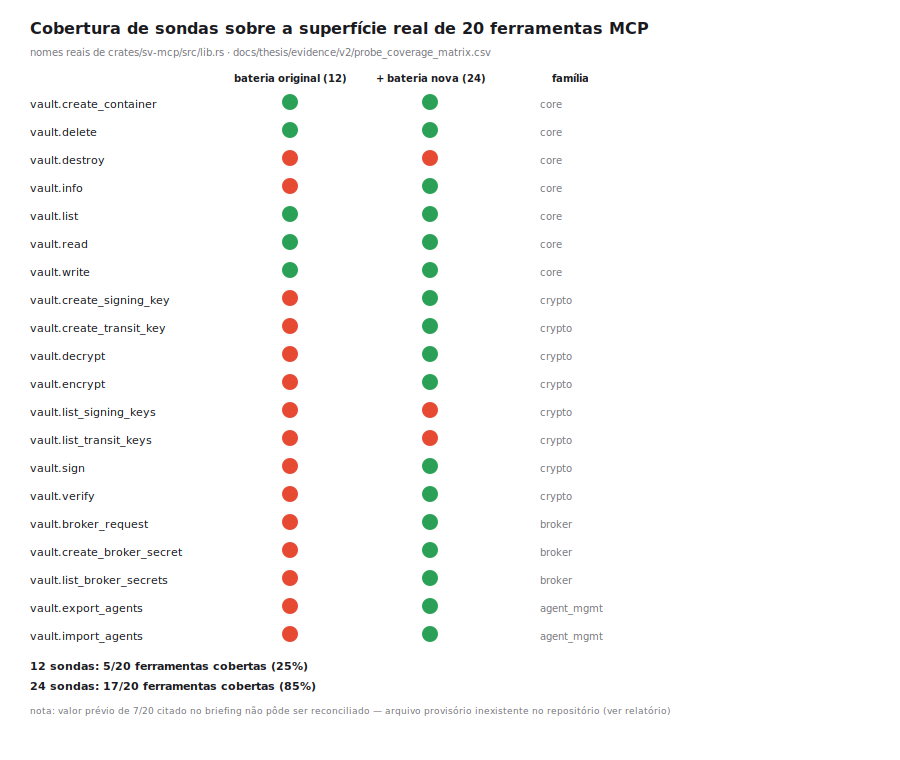
\includegraphics[width=0.85\textwidth]{figuras/cobertura_sondas.png}
\fonte{Elaboração própria a partir de \codigo{docs/thesis/evidence/v2/probe_coverage_matrix.csv}.}
\end{figure}

As sondas A11--A15 confirmam a correção \textit{fail-closed} de criptografia e corretagem, descrita na \hyperref[nota:headless]{nota de segurança do modo \textit{headless}}, contra o binário real compilado, dirigido como subprocesso, e não contra uma política espelhada em código de teste. É essa distinção que torna o resultado evidência sobre o artefato, e não sobre uma reimplementação da sua política. Dos 12 vereditos pré-especificados da extensão, 11 corresponderam ao observado, e a cadeia de auditoria HMAC das execuções foi verificada (12 entradas, \codigo{verify_chain}). O único desvio é objeto da subseção seguinte. Seguindo o critério já adotado neste capítulo, o resultado é reportado como contagens sobre a bateria executada, e não como taxa percentual de sucesso.

\subsection{Defeito Revelado pela Sonda C4}
\label{sec:defeito-c4}
A sonda C4, cujo veredito esperado foi congelado antes da execução, revelou um defeito real do artefato: \codigo{enforce_scopes} nega incondicionalmente \codigo{vault.info}, \codigo{vault.export_agents} e \codigo{vault.import_agents} para qualquer agente com escopos definidos, tornando essas operações inalcançáveis no modo \textit{headless} real, enquanto a política \textit{headless} pretendida permite \codigo{vault.info} como consulta de metadados. O desvio entre o veredito pré-especificado e o observado não é tratado como falha da avaliação, e sim como resultado dela: uma sonda pré-especificada que falha e, com isso, expõe um defeito real é a evidência mais forte disponível de que estender a bateria era metodologicamente necessário. Um defeito encontrado por uma sonda cuja expectativa fosse escrita após a execução valeria muito menos, pois não excluiria acomodação \textit{post-hoc} da expectativa ao comportamento observado. O achado é, portanto, uma contribuição do desenho da avaliação; a correção do defeito consta dos trabalhos futuros.

\section{Síntese dos Resultados}
O artefato concretiza, no domínio de segredos e credenciais, os quatro módulos da arquitetura de referência apresentados na Figura~\ref{fig:arquitetura-referencia}: cofre local cifrado, servidor MCP local, mediação com filtro de privacidade, modos de consentimento e auditoria implementados. A sequência da Figura~\ref{fig:fluxo-requisicao} explicita que autenticação, validação e escopo antecedem a operação no cofre, enquanto consentimento e filtragem dependem do modo configurado. Essa separação é lógica e não constitui isolamento de processo ou de sistema operacional.

A síntese empírica permanece subordinada à Tabela~\ref{tab:fronteira-evidencia}. Sob o protocolo corrigido, a Tabela~\ref{tab:latencia-pareada-v2} mostra que nenhum dos seis contrastes pareados entre DIRECT e os modos de consentimento exclui zero, e a Figura~\ref{fig:latencia-estagios} mostra que o filtro de PII domina a condição ANONYMIZED de maior carga. A medição de escopos no caminho \textit{WebSocket} observa diferenças entre 2,1 e 2,2\micro{} com 20 escopos, sob ordem fixa dos braços, sem separar o efeito de escopo do efeito de posição (Tabela~\ref{tab:enforce-scopes}). A bateria da Tabela~\ref{tab:sondas-adversariais} bloqueia 10/10 chamadas maliciosas e aceita 2/2 controles; sua extensão a 24 sondas eleva a cobertura da superfície de ferramentas de 5/20 para 17/20 e revela o defeito da Seção~\ref{sec:defeito-c4}. O conjunto valida somente as negativas enumeradas no transporte \textit{WebSocket}, com escopo, caminho e política HITL simulada.

Em conjunto, os resultados mostram que a instância permite observar mediação de leituras nomeadas, decompor a latência interna do \textit{gateway} e exercitar uma bateria finita de acessos laterais. Não se obtém desses dados evidência sobre experiência fim a fim, comportamento de um adversário adaptativo, comparação com nuvem, retenção no provedor ou identificabilidade de documentos. Tampouco se avaliam RAG, índice vetorial ou isolamento de memória no sistema operacional.

\section{Respostas às Questões de Pesquisa}
\subsection{QP1}
A mediação de leituras nomeadas ocorre pela combinação de identidade autenticada, escopos de capacidade, validação de caminhos, modos de contêiner e registro de auditoria. No caminho \textit{desktop}, APPROVAL e OTP submetem a liberação ao consentimento configurado, enquanto ANONYMIZED aplica mascaramento heurístico à saída textual. A auditoria encadeada por HMAC-SHA256 fornece evidência de adulteração, remoção e truncamento em relação ao ponto de verificação local presente, sem impedir a restauração de uma cópia completa e internamente consistente. A evidência experimental de escopo e consentimento refere-se ao \textit{gateway desktop WebSocket}; o modo \textit{headless} fica excluído dessa avaliação e, embora preserve escopos e recuse operações secretas sem modelo de consentimento, não oferece consentimento humano.

A redução de exposição sustentada pela evidência é, portanto, operacional e delimitada: escopos restringem as chamadas alcançáveis e o modo ANONYMIZED mascara as categorias detectadas antes da saída. \textit{Contêineres} DIRECT liberam leituras sem consentimento por projeto e ficam fora da garantia de mediação humana, embora permaneçam sujeitos aos demais controles aplicáveis. O filtro cobre exatamente sete categorias heurísticas, mas as cargas sintéticas ANONYMIZED do \textit{microbenchmark} exercitam somente e-mail, CPF e IPv4. Na caracterização dedicada do filtro, o \textit{recall} em forma canônica é de 100\% nas sete categorias documentadas (200/200 por categoria), com 0\% de falso positivo em texto neutro (0/500 por categoria); a robustez fora da forma canônica varia por categoria, como detalhado na resposta à QP2.

Essa resposta não equivale a garantia de anonimização ou de não identificabilidade. RG, CEP, nomes completos, endereços, datas de nascimento e telefones sem formatação não são detectados, e a presença combinada desses campos, em especial nome e endereço, é precisamente o que pode sustentar a identificabilidade referida no Art.~5º da LGPD, mantendo um documento identificável mesmo quando CPF ou CNPJ são mascarados. O resultado também não estabelece conformidade à LGPD.

\subsection{QP2}
Sob o protocolo corrigido, a resposta à QP2 no limite do caminho local instrumentado é que nenhum dos seis IC de 95\% do contraste entre medianas da Tabela~\ref{tab:latencia-pareada-v2} exclui zero sob \textit{AutoAllow}, sem que isso constitua teste de equivalência, e a latência total medida permanece abaixo de um milissegundo em todas as condições. A medição de escopos no caminho \textit{WebSocket} observa diferenças entre 2,1 e 2,2\micro{} com 20 escopos, sob ordem fixa dos braços, que não separa o efeito do tamanho do conjunto do efeito da posição de execução (Tabela~\ref{tab:enforce-scopes}). A exceção relevante é o filtro de PII, cujo custo cresce com o conteúdo sintético e domina a leitura ANONYMIZED de 16 KiB; as medições isoladas e internas ao gateway não devem ser somadas como uma nova latência fim a fim.

A Tabela~\ref{tab:metodologia-microbenchmark} delimita o estimando: o transporte \textit{stdio} mede validação de parâmetros e caminho, despacho, leitura/decifra e filtragem quando aplicável, mas não mede resolução de agente nem \codigo{enforce_scopes}, medido à parte no \textit{WebSocket}. O total instrumentado soma estágios e exclui a escrita de auditoria (Seção~\ref{sec:fronteira-evidencia}), e os valores dependem da máquina hospedeira. Não se mede a chamada MCP fim a fim, WAN, inferência, utilidade de tarefa ou tempo de decisão humana; APPROVAL e OTP usam \codigo{AutoAllow} e representam somente o piso mecânico do \textit{gateway}.

A caracterização dedicada do filtro de privacidade real (\codigo{sv-privacy}) qualifica a QP2 em duas direções. Primeiro, a robustez a formato não é uniforme: ela é por categoria (Tabela~\ref{tab:pii-robustez}). CPF, CNPJ e cartão compartilham o mecanismo \codigo{collect_grouped_digits} e são 100\% robustos à variação de pontuação; telefone, SSN e e-mail exigem sintaxe fixa e caem a 0\% fora da forma canônica, com a exceção do formato internacional \codigo{+55}, que é detectado. A formulação honesta é que as três categorias portadoras de dígito verificador ou soma de verificação são robustas a formato, e as três de sintaxe fixa não são.

\begin{table}[htb]
\centering
\small
\caption{Recall do filtro de privacidade real (\texttt{sv-privacy}) por categoria e por formato. Todos os identificadores são sintéticos (RFC 1918, RFC 2606, bloco NANP 555-01XX, faixa SSN 900--999, BIN de teste 400000).}
\label{tab:pii-robustez}
\begin{tabular}{@{}llll@{}}
\toprule
Categoria & Canônico & Não canônico & Mecanismo no código \\
\midrule
CPF               & 100\% & 100\% & \multirow{3}{*}{\texttt{collect\_grouped\_digits}: robusto} \\
CNPJ              & 100\% & 100\% & \\
Cartão (Luhn)     & 100\% & 100\% & \\
\midrule
IPv4              & 98\%  & 0\% espaçado; 93\% CIDR & sintaxe pontuada \\
Telefone          & 100\% & 0\% sem símbolo; 100\% \texttt{+55} & exige \texttt{+} ou \texttt{(} \\
SSN               & 100\% & 0\%   & exige hífen exato \\
E-mail            & 100\% & 0\%   & sem tolerância a espaçamento \\
\midrule
\multicolumn{4}{@{}p{\dimexpr\linewidth-10\tabcolsep\relax}@{}}{\emph{Lacunas admitidas} (RG, CEP, nome, endereço, data de nascimento,
telefone não formatado): 0\% --- sem detector.} \\
\bottomrule
\end{tabular}
\fonte{\codigo{docs/thesis/evidence/v2/pii_format_robustness.csv}.}
\end{table}

Segundo, o custo do filtro é dominado pela densidade de PII no documento, e não pela varredura do texto: a densidade responde por 63,7\% da inclinação marginal do custo ($R^2=0{,}99979$ no ajuste tamanho~$\times$~densidade). O ajuste novo, avaliado na densidade máxima testada, reproduz 97,0\% da inclinação do \codigo{micro.csv} publicado (7,395 contra 7,626~ns/B); essa concordância é compatível com a medição preliminar, mas não identifica, por si só, a composição da carga antiga. A inclinação estimada para documentos sem PII é de 2,68~ns/B, aproximadamente 35,2\% da inclinação publicada de 7,63~ns/B. Os valores caracterizam as densidades sintéticas exercitadas e não estabelecem custo típico de documentos reais nem limite superior universal.

\subsection{QP3}
No modelo de ameaça de usuário único e máquina única, a bateria pré-especificada na Tabela~\ref{tab:sondas-adversariais} fornece evidência de que, sobre transporte \textit{WebSocket} autenticado, o protocolo composto por escopos, validação de caminho e política HITL simulada bloqueia as chamadas maliciosas enumeradas e preserva os dois controles legítimos. A execução não isola a contribuição causal de cada controle nem avalia isoladamente a autenticação. O resultado de 10/10 sondas maliciosas bloqueadas e 2/2 controles aceitos é uma cobertura da bateria executada, não uma taxa populacional de ataques ou uma prova de robustez geral. A extensão da bateria eleva a cobertura da superfície de ferramentas de 5/20 para 17/20, confirma contra o binário real, dirigido como subprocesso, a correção \textit{fail-closed} de criptografia e corretagem (sondas A11--A15, com 11 dos 12 vereditos pré-especificados correspondendo ao observado e cadeia de auditoria verificada) e revela o defeito de imposição de escopos da Seção~\ref{sec:defeito-c4}.

A execução ocorre uma única vez sobre \textit{WebSocket} autenticado e usa \codigo{HitlPolicy} simulada; o controlador \textit{desktop} real \codigo{ApprovalState} não é exercitado. Também não se atribui cada bloqueio individual a uma causa observada, não se testa adversário adaptativo e não se avalia exfiltração por operações permitidas. Assim, a resposta à QP3 restringe-se ao protocolo e às negativas enumeradas.

\section{Confronto com os Trabalhos Correlatos}
O posicionamento apresentado na Tabela~\ref{tab:posicionamento-correlatos} é retomado nesta seção para confrontar funções arquiteturais, sem converter diferenças de etapa ou domínio em comparação de desempenho, privacidade ou segurança. A linha do \textit{Sovereign Vault} deve ser lida no modelo de ameaça declarado na metodologia: usuário único, máquina única e agente MCP autenticado e potencialmente comprometido, sem isolamento de processo ou de sistema operacional.

O Aprendizado Federado preserva a descentralização de dados brutos durante o treinamento cooperativo de modelos \cite{mcmahan2017,mammen2021}, enquanto o problema aqui tratado é o acesso, em tempo de execução, a segredos e credenciais locais voláteis. O \textit{Sovereign Vault} não substitui essa abordagem: atua em outra etapa do ciclo, mediando chamadas de ferramenta e limitando a saída de dados nomeados. A avaliação realizada não compara desempenho, privacidade ou utilidade entre as duas abordagens.

\textit{Solid} descentraliza o armazenamento pessoal em \textit{pods} e organiza dados segundo semântica voltada à \textit{Web} \cite{sambra2016}. A contribuição desta instanciação concentra-se, em contraste, no \textit{gateway} MCP local que combina escopo, consentimento, transformação de saída e auditoria para leituras nomeadas. O contraste delimita funções arquiteturais, mas não demonstra superioridade sobre \textit{Solid}, pois não há experimento comparativo.

HAMSTER/Sphere converge estruturalmente com o \textit{Sovereign Vault} ao concentrar autenticação em um ponto de controle anterior à operação \cite{pigatto2016}. Diverge, contudo, quanto ao domínio, ao objeto protegido e ao modelo de falha: a negação por padrão do HAMSTER não equivale à autorização por escopos do \textit{Sovereign Vault}, na qual escopos vazios representam superfície irrestrita ainda sujeita ao modo do \textit{contêiner}. Não se executa experimento comparativo entre as arquiteturas, e a correspondência não equipara os modos de \textit{contêiner} do \textit{Sovereign Vault} às categorias de criticidade de HAMSTER.

Desse modo, a contribuição situa-se na mediação operacional entre agentes e dados locais, de forma complementar à descentralização de treinamento e de armazenamento. Essa posição permanece restrita ao domínio avaliado de segredos e credenciais. A generalização para documentos e recuperação semântica ainda não é demonstrada.

\section{Considerações Finais}

Neste capítulo são apresentados os resultados da avaliação do artefato, sempre subordinados à fronteira de evidência fixada na Seção~\ref{sec:fronteira-evidencia}. Sob o protocolo corrigido, o \textit{microbenchmark} indica que nenhum dos seis IC de 95\% do contraste entre medianas exclui zero sob \textit{AutoAllow}, sem que isso constitua teste de equivalência; a medição separada no caminho \textit{WebSocket} observa diferenças entre 2,1 e 2,2\micro{} para 20 escopos, sob ordem fixa dos braços, sem isolar esse efeito da posição de execução; a caracterização do filtro de privacidade separa \textit{recall} canônico de robustez a formato, que não é uniforme entre as categorias; e a bateria adversarial pré-especificada, ampliada de 5/20 para 17/20 ferramentas da superfície MCP, expõe um defeito real de imposição de escopos no modo \textit{headless}. As respostas às questões de pesquisa e o confronto com os trabalhos correlatos são construídos estritamente sobre esses dados, preservando as qualificações que cada alegação exige. Sendo assim, no próximo capítulo são apresentadas as conclusões do trabalho, com as contribuições, as limitações e os trabalhos futuros.

\chapter{CONCLUSÕES}
Este capítulo retoma o percurso da pesquisa à luz dos resultados obtidos e consolida o que o trabalho entrega. As contribuições são organizadas segundo a taxonomia de March e Smith \cite{march1995}, já adotada no percurso metodológico; em seguida são explicitadas as limitações que delimitam o alcance das alegações e indicados os desdobramentos que a evidência disponível torna prioritários.

\section{Contribuições}
As contribuições organizam-se segundo a taxonomia de March e Smith \cite{march1995}, já adotada no percurso metodológico. A organização distingue o desenho abstrato, o procedimento de mediação e sua concretização executável, evitando atribuir à instanciação capacidades previstas apenas na visão arquitetural. A forma da contribuição, arquitetura nomeada, com camada de segurança explícita e acompanhada de estudos de caso avaliativos, segue precedente estabelecido em arquiteturas de segurança para sistemas críticos \cite{pigatto2016}; nesta instanciação, porém, a avaliação permanece artificial e somativa: a latência usa dez sessões sob o protocolo corrigido, com IC de 95\% por \textit{bootstrap}, enquanto as baterias adversariais permanecem execuções finitas, sem inferência de taxa populacional.

\begin{itemize}
\item \textbf{Modelo}: arquitetura de referência \textit{Local-First} em quatro módulos, com uma fronteira lógica entre o agente externo e os quatro módulos locais: cofre, \textit{gateway}, mediação e auditoria. O modelo é concretizado no domínio de segredos e credenciais e não inclui isolamento de memória no SO, RAG ou índice vetorial na instância avaliada.
\item \textbf{Método}: protocolo que autentica, valida, aplica escopos e o consentimento configurado, executa localmente, filtra a saída ANONYMIZED quando aplicável e registra a operação. Sua avaliação é artificial e somativa, limitada aos caminhos e às condições instrumentadas.
\item \textbf{Instanciação}: protótipo \textit{Sovereign Vault} e \textit{harness} que produzem evidência rastreável de latência interna e das sondas pré-especificadas. A instanciação integra armazenamento cifrado, \textit{gateway} MCP, modos de consentimento, filtro heurístico e auditoria com evidência de adulteração, com as qualificações da Tabela~\ref{tab:fronteira-evidencia}.
\end{itemize}

Há ainda uma contribuição metodológica na documentação do ciclo construir--avaliar por ADRs. A observação de que o modo reservado NATIVE podia degradar para acesso sem solicitação de consentimento conduz à correção do mecanismo de consentimento e à inclusão das sondas A9 e A10 na bateria. Esse encadeamento registra achado, decisão, correção e ampliação da avaliação sem converter a bateria finita em prova geral de segurança.

\section{Limitações}
A validade externa é limitada pelo enquadramento artificial e somativo. A evidência de desempenho do \textit{gateway} provém do protocolo corrigido ($k=10$ sessões, mediana com IC de 95\% por \textit{bootstrap}), mas permanece sintética e dependente da máquina hospedeira; não inclui latência fim a fim, WAN, inferência, carga de produção, utilidade de tarefa ou decisão humana, e o total instrumentado soma estágios e exclui a escrita de auditoria (Seção~\ref{sec:fronteira-evidencia}). O caminho \textit{stdio} não cronometra resolução de agente nem aplicação de escopos; o custo de \codigo{enforce_scopes} foi medido à parte, no caminho \textit{WebSocket} (Tabela~\ref{tab:enforce-scopes}), com a ressalva de ordem fixa dos \textit{ARM} de escopo registrada na nota daquela tabela.

A bateria adversarial é finita e pré-especificada. Ela exercita chamadas de ferramenta, e não um LLM submetido a \textit{prompt injection}; a política HITL é simulada e o controlador real de consentimento \textit{desktop} não é exercitado, embora as sondas A11--A15 da extensão dirijam o binário real compilado como subprocesso; e não cobre adversário adaptativo, \textit{fuzzing} da superfície JSON-RPC ou exfiltração por caminhos permitidos. Após a extensão, três ferramentas permanecem sem cobertura: \codigo{vault.destroy}, \codigo{vault.list_transit_keys} e \codigo{vault.list_signing_keys}. O resultado não permite estimar taxa populacional nem atribuir causalmente cada bloqueio a um controle específico.

O artefato restringe-se a um usuário, uma máquina e segredos ou credenciais acessados por nome. Processos sob a mesma conta, comprometimento do sistema operacional, inspeção de memória, dependências nativas e roubo de \textit{token} ficam fora do limite avaliado; a separação entre \textit{contêineres} é lógica, com uma única DEK ativa e sem isolamento por chave. \textit{Contêineres} DIRECT dispensam consentimento por projeto, e a correção \textit{fail-closed} do \hyperref[nota:headless]{modo \textit{headless}} não transforma o modo \textit{headless} em caminho de consentimento humano. Pareamento, resolução de agente, aplicação de escopo e consentimento valem exclusivamente para o transporte \textit{WebSocket} autenticado: iniciar o binário no transporte \textit{stdio} opera com \codigo{PairState::AlreadyPaired(None)} e, portanto, sem resolução de agente nem \codigo{enforce_scopes} (\codigo{crates/sv-mcp/src/lib.rs:1003,1303}). Isso não é uma falha do mecanismo, e sim consequência do limite declarado: quem pode iniciar o processo já detém acesso local sob a mesma conta do usuário, condição situada fora do modelo de ameaça. A sequência de autenticação, validação e escopo da Figura~\ref{fig:fluxo-requisicao} descreve, assim, o caminho \textit{WebSocket}, e é a esse caminho que se referem os resultados da bateria adversarial.

O uso sem retorno de bytes de chave não elimina o risco de o \textit{gateway} atuar como oráculo criptográfico, pois a autorização não está vinculada à referência de chave, ao \textit{hash} do \textit{payload}, à semântica da operação, ao destinatário ou domínio e à identidade do agente. A auditoria detecta alteração em relação ao ponto de verificação local presente, mas não uma restauração completa e coerente do diretório. Nomes lógicos, modos, tamanhos e outros metadados também podem permanecer visíveis.

O filtro ANONYMIZED opera somente sobre texto e cobre sete categorias heurísticas; o \textit{recall} e a taxa de falso positivo foram medidos por categoria e formato sobre identificadores sintéticos (Tabela~\ref{tab:pii-robustez}), o que não estabelece desempenho sobre documentos reais. Campos brasileiros relevantes, como RG, CEP, nomes e endereços, permanecem fora da detecção, assim como datas de nascimento e telefones sem formatação. Por isso, mascaramento parcial não implica anonimização, não identificabilidade ou conformidade à LGPD. Uma caracterização adicional usa um corpus sintético mantido fora deste repositório, com 48 casos no total, dos quais oito são controles negativos. O adaptador invoca \codigo{sv_privacy::redact} diretamente, sem \textit{gateway}, autenticação ou auditoria. Nos 14 casos canônicos, dois por categoria coberta, são registrados 14 acertos; nos oito controles negativos não há achados. Nas cinco categorias sem detector correspondente -- nome de pessoa, endereço, data de nascimento, CEP e segredo genérico -- são registrados zero acertos em dois casos por categoria, sob correspondência exata de categoria e \textit{span}. A amostra sintética caracteriza esses casos e não estabelece taxa populacional sobre documentos reais. As observações, os escores, seus resumos criptográficos e a declaração de procedência estão em \codigo{docs/thesis/evidence/v3/pii-externa/}; a reprodução integral requer também o corpus rotulado e o código do adaptador identificado nessa declaração. Essa separação espelha uma lição da literatura de sistemas críticos: propriedades de \textit{safety} e de \textit{security} não se implicam mutuamente, e arquiteturas projetadas para satisfazer uma podem conter lacunas na outra, o que exige tratamento conjunto desde o projeto \cite{ferrao2022}. Analogamente, garantir uma propriedade técnica, escopos, consentimento, mascaramento, e satisfazer uma qualificação jurídica como a do Art.~5º da LGPD são exigências distintas, que divergem exatamente nos campos que o filtro não detecta.

As dez sessões registradas da reavaliação E1 usam o protocolo corrigido de ordem e aquecimento, mas seus metadados não documentam o intervalo mínimo entre execuções nem o bloqueio do modo de energia previstos para a execução definitiva: os dez arquivos de proveniência registram início entre 18h17min16s e 18h17min38s do mesmo dia, e o modo de energia consta como não fixável no hospedeiro. Os intervalos de confiança por reamostragem de sessões descrevem essa coleta e não eliminam possível dependência de estado entre execuções.

Por fim, não há braço de comparação em nuvem, verificação de retenção ou descarte pelo provedor, \textit{contêineres} de contexto, busca semântica ou \textit{embeddings} locais. Essas ausências impedem responder por superioridade perante uma arquitetura em nuvem e por generalização da instanciação para documentos. Elas definem a agenda de continuidade, e não capacidades implícitas do protótipo atual.

\section{Trabalhos Futuros}
A avaliação de latência do \textit{gateway} foi reexecutada sob protocolo corrigido, com $k=10$ sessões, IC de 95\% por \textit{bootstrap} e descarte explícito de aquecimento (Tabela~\ref{tab:latencia-pareada-v2}), e a influência da densidade de PII sobre o custo do filtro foi quantificada na linha da avaliação por fatores de Silva et al. \cite{silva2016}. Permanecem prioridades empíricas: instrumentar a escrita de auditoria como um quinto estágio de \codigo{StageTimings}, hoje excluída do total reportado; preservar os metadados já coletados em E1 e cumprir, em nova execução, o controle de energia e o intervalo entre sessões previstos no protocolo definitivo; e aleatorizar a ordem dos braços de escopo, cuja ordem fixa impede separar os efeitos de escopo e de posição, como ilustra o delta negativo registrado na nota da Tabela~\ref{tab:enforce-scopes}.

O protocolo de dois braços deve comparar o mesmo modelo e versão com acesso ao material sintético pelo \textit{gateway} local e por um caminho de contexto em nuvem, com telemetria, \textit{baseline}, governança e plano estatístico definidos antes da execução. Em complemento, um estudo com participantes deve medir mediana, p95, \textit{timeouts} e negações do tempo de decisão humana para APPROVAL e OTP. Esses estudos permitem avaliar comparação e experiência, mas a retenção ou o descarte no provedor exige verificação própria e não decorre automaticamente do protocolo.

A bateria de segurança deve incorporar o controlador \textit{desktop} real, registro causal por sonda, adversário adaptativo, casos de exfiltração por operações permitidas e testes de entradas JSON-RPC malformadas ou superdimensionadas. Cabe também corrigir o defeito revelado pela sonda C4, alinhar \codigo{enforce_scopes} à política \textit{headless} pretendida, que permite \codigo{vault.info}, e cobrir as três ferramentas restantes: \codigo{vault.destroy}, \codigo{vault.list_transit_keys} e \codigo{vault.list_signing_keys}. \textit{Fuzzing} e execuções independentes ampliam a cobertura observada, sem converter resultados finitos em garantia universal. O tratamento do \textit{token} também deve migrar para arquivo com permissão 0600 ou chaveiro do sistema operacional.

O classificador determinístico de sensibilidade e consentimento adaptativo descrito no ADR-0013 permanece proposto e não implementado. Antes de qualquer alegação de eficácia, requer implementação com elevação apenas, falha fechada e limites de complexidade, além de conjunto rotulado, pré-registro dos pisos de precisão e \textit{recall}, separação entre calibração e teste e sondas sobre \textit{WebSocket} autenticado. Resultado abaixo dos pisos deve ser reportado como negativo, pois o mecanismo constitui uma rede de segurança de usabilidade para exposição acidental, e não um controle de segurança contra agente com escrita.

Os detectores de PII devem ser ampliados e avaliados para dados brasileiros, incluindo RG, CEP, nomes e endereços, com precisão e \textit{recall} por categoria em conjunto rotulado. Detectores ambíguos, entendidos aqui como aqueles sem validação por dígito verificador ou soma de verificação e, por isso, sujeitos a maior taxa de falsos positivos, devem permanecer fora da elevação adaptativa até satisfazerem critério pré-especificado, e desempenho sintético deve conservar a ressalva de validade externa. Essa linha de trabalho reduz lacunas conhecidas do mascaramento, mas não estabelece conformidade à LGPD.

Na camada criptográfica, a autorização deve ser vinculada à chave e ao uso pretendido, incluindo \textit{hash} do \textit{payload}, semântica da operação, destinatário ou domínio e identidade do agente. Também cabe introduzir hierarquia de chaves por \textit{contêiner} ou manter explicitamente a segmentação apenas lógica e avaliar controles de SO em múltiplas plataformas. Para a auditoria, uma âncora externa confiável, como registro de transparência remoto ou contador monotônico protegido, deve permitir distinguir restauração integral de continuidade legítima.

Os \textit{contêineres} de contexto descritos no ADR-0012 também permanecem propostos e não implementados. Sua avaliação futura abrange documentos textuais, índice vetorial e \textit{embeddings} no dispositivo, busca aproximada e filtragem de trechos recuperados antes da saída pelo \textit{gateway}. Essa extensão exige protocolo próprio de latência, cobertura adversarial da nova superfície e tratamento explícito do ciclo de vida do índice; somente depois desses resultados é possível discutir RAG como capacidade do artefato.

\postextual
\begin{thebibliography}{99}
\bibitem{nisa2025} NISA, Ume et al. Agentic AI: the age of reasoning -- a review. \textit{Journal of Automation and Intelligence}, v. 5, n. 1, p. 69-89, mar. 2026. DOI: 10.1016/j.jai.2025.08.003.
\bibitem{vaswani2017} VASWANI, Ashish et al. Attention is all you need. In: \textit{ADVANCES IN NEURAL INFORMATION PROCESSING SYSTEMS (NEURIPS)}, 2017, Long Beach. Proceedings [...]. p. 5998-6008.
\bibitem{liu2024} LIU, Xiao et al. AgentBench: evaluating LLMs as agents. In: \textit{INTERNATIONAL CONFERENCE ON LEARNING REPRESENTATIONS (ICLR)}, 2024, Vienna. Proceedings [...]. 2024. arXiv:2308.03688.
\bibitem{wu2011} WU, Wei-Wen. Developing an explorative model for SaaS adoption. \textit{Expert Systems with Applications}, v. 38, n. 12, p. 15057-15064, 2011. DOI: 10.1016/j.eswa.2011.05.039.
\bibitem{zuboff2019} ZUBOFF, Shoshana. \textit{The age of surveillance capitalism: the fight for a human future at the new frontier of power}. New York: PublicAffairs, 2019.
\bibitem{anthropic2024} ANTHROPIC PBC. \textit{Model Context Protocol Specification}. v. 1.0. 2024. Disponível em: \url{https://modelcontextprotocol.io}. Acesso em: 10 abr. 2026.
\bibitem{kleppmann2019} KLEPPMANN, Martin et al. Local-first software: you own your data, in spite of the cloud. In: \textit{ACM SIGPLAN SYMPOSIUM (ONWARD!)}, 2019, Athens. Proceedings [...]. New York: ACM, 2019. p. 154-178. DOI: 10.1145/3359591.3359737.
\bibitem{khan2022} KHAN, Salman et al. Transformers in vision: a survey. \textit{ACM Computing Surveys}, v. 54, n. 10s, p. 1-41, 2022. DOI: 10.1145/3505244.
\bibitem{lewis2020} LEWIS, Patrick et al. Retrieval-augmented generation for knowledge-intensive NLP tasks. In: \textit{ADVANCES IN NEURAL INFORMATION PROCESSING SYSTEMS (NEURIPS)}, 33., 2020. Proceedings [...]. p. 9459-9474.
\bibitem{sakar2024} ŞAKAR, Tolga; EMEKÇI, Hakan. Maximizing RAG efficiency: a comparative analysis of RAG methods. \textit{Natural Language Processing}, v. 31, n. 1, p. 1-25, jan. 2025. DOI: 10.1017/nlp.2024.53.
\bibitem{lorenzon2021} LORENZON, Laila Neves. Análise comparada entre regulamentações de dados pessoais no Brasil e na União Europeia (LGPD e GDPR) e seus respectivos instrumentos de enforcement. \textit{Revista do Programa de Direito da União Europeia}, v. 1, p. 39-52, 2021. Disponível em: \url{https://periodicos.fgv.br/rpdue/article/view/83423}. Acesso em: 22 set. 2026.
\bibitem{cavoukian2011} CAVOUKIAN, Ann. \textit{Privacy by Design: the 7 foundational principles}. Toronto: Information and Privacy Commissioner of Ontario, 2011.
\bibitem{nsa2022} NATIONAL SECURITY AGENCY. \textit{Software Memory Safety: Cybersecurity Information Sheet}. 2022. Disponível em: \url{https://media.defense.gov/2022/Nov/10/2003112742/-1/-1/0/CSI_SOFTWARE_MEMORY_SAFETY.PDF}. Acesso em: 1 jun. 2026.
\bibitem{mcmahan2017} MCMAHAN, Brendan et al. Communication-efficient learning of deep networks from decentralized data. In: \textit{INTERNATIONAL CONFERENCE ON ARTIFICIAL INTELLIGENCE AND STATISTICS}, 20., 2017. Proceedings [...]. [S.l.]: PMLR, 2017. p. 1273-1282. (Proceedings of Machine Learning Research, v. 54). Disponível em: \url{https://proceedings.mlr.press/v54/mcmahan17a.html}. Acesso em: 4 ago. 2026.
\bibitem{mammen2021} MAMMEN, Priyanka Mary. Federated learning: opportunities and challenges. \textit{arXiv preprint arXiv:2101.05428}, 2021. DOI: 10.48550/arXiv.2101.05428.
\bibitem{sambra2016} SAMBRA, Andrei Vlad et al. \textit{Solid: a platform for decentralized social applications based on linked data}. Cambridge: MIT CSAIL, 2016. (Technical Report).
\bibitem{pigatto2016} PIGATTO, Daniel Fernando et al. The HAMSTER data communication architecture for unmanned aerial, ground and aquatic systems. \textit{Journal of Intelligent \& Robotic Systems}, v. 84, p. 705-723, 2016. DOI: 10.1007/s10846-016-0356-x.
\bibitem{simon1996} SIMON, Herbert A. \textit{The sciences of the artificial}. 3. ed. Cambridge, MA: MIT Press, 1996.
\bibitem{hevner2004} HEVNER, Alan R. et al. Design science in information systems research. \textit{MIS Quarterly}, v. 28, n. 1, p. 75-105, 2004. DOI: 10.2307/25148625.
\bibitem{hevner2007} HEVNER, Alan R. A three cycle view of design science research. \textit{Scandinavian Journal of Information Systems}, v. 19, n. 2, p. 87-92, 2007.
\bibitem{venable2016} VENABLE, John; PRIES-HEJE, Jan; BASKERVILLE, Richard. FEDS: a framework for evaluation in design science research. \textit{European Journal of Information Systems}, v. 25, n. 1, p. 77-89, 2016. DOI: 10.1057/ejis.2014.36.
\bibitem{peffers2007} PEFFERS, Ken et al. A design science research methodology for information systems research. \textit{Journal of Management Information Systems}, v. 24, n. 3, p. 45-77, 2007. DOI: 10.2753/MIS0742-1222240302.
\bibitem{march1995} MARCH, Salvatore T.; SMITH, Gerald F. Design and natural science research on information technology. \textit{Decision Support Systems}, v. 15, n. 4, p. 251-266, 1995. DOI: 10.1016/0167-9236(94)00041-2.
\bibitem{rfc2606} EASTLAKE, Donald; PANITZ, Aliza. \textit{Reserved Top Level DNS Names}. RFC 2606, 1999. Disponível em: \url{https://www.rfc-editor.org/rfc/rfc2606}. Acesso em: 3 ago. 2026.
\bibitem{rfc1918} REKHTER, Yakov et al. \textit{Address Allocation for Private Internets}. Request for Comments (RFC) 1918, 1996. Disponível em: \url{https://www.rfc-editor.org/rfc/rfc1918}. Acesso em: 3 ago. 2026.
\bibitem{silva2016} SILVA, Natassya Barlate Floro da et al. Case studies of performance evaluation of cryptographic algorithms for an embedded system and a general purpose computer. \textit{Journal of Network and Computer Applications}, v. 60, p. 130-143, 2016. DOI: 10.1016/j.jnca.2015.10.007.
\bibitem{ferrao2022} FERRÃO, Isadora Garcia et al. Security and safety concerns in air taxis: a systematic literature review. \textit{Sensors}, v. 22, n. 18, art. 6875, 2022. DOI: 10.3390/s22186875.
\end{thebibliography}

\begin{apendicesenv}
\chapter{REPRODUTIBILIDADE DA EVIDÊNCIA ATUAL}
\label{cap:reprodutibilidade}

{\sloppy \textbf{Disponibilidade.} O repositório do projeto é público em \url{https://github.com/pealmeida/sovereign-vault}, sob licença Apache 2.0, e reúne o código-fonte do protótipo, a evidência bruta, os agregados e os \textit{scripts} de verificação citados neste trabalho. As citações de código na forma \codigo{arquivo:linhas} referem-se à árvore fixada pela etiqueta anotada \codigo{thesis-code-reference-2026-09-22}, correspondente ao \textit{commit} \codigo{ec3bd73ec}, que é a referência a ser usada para localizá-las. O ramo \codigo{main} seguiu evoluindo depois dessa marcação, de modo que as mesmas faixas de linha podem apontar para conteúdo distinto nele; a etiqueta permanece alcançável por \codigo{git fetch --tags} independentemente disso. Acesso em: 22 set. 2026.\par}
Os artefatos analisados estão versionados em \codigo{docs/thesis/evidence/}, nos arquivos \codigo{latency.csv}, \codigo{adversarial.csv} e \codigo{micro.csv}. São cópias fiéis, verificadas por resumo criptográfico, da saída gerada em \codigo{target/thesis-eval/}, diretório que não é versionado. O comando registrado para produzir a execução preliminar de desenvolvimento é:
\begingroup
\footnotesize
\begin{verbatim}
cargo run --release -p thesis-eval -- all --out target/thesis-eval --iterations 1000
\end{verbatim}
\endgroup
A execução preliminar foi produzida a partir do \textit{commit} sanitizado \codigo{8cea41adae5e}, alcançável pela etiqueta anotada \codigo{thesis-evidence-preliminary}. A reescrita de proveniência preservou, byte a byte, os subdiretórios de código exercitados pelo protocolo e os três CSVs versionados; seu registro está em \codigo{docs/HISTORY-SANITIZATION.md}. Esse \textit{commit} não é ancestral do ramo principal: o código instrumentado evoluiu depois dele, de modo que os números aqui reportados correspondem a um estado anterior ao da versão entregue, coerentemente com sua classificação como execução preliminar. A execução definitiva será produzida a partir de um estado publicado do ramo principal e receberá etiqueta própria. O perfil é \codigo{release}; a plataforma registrada na documentação de avaliação (\codigo{docs/thesis/EVALUATION.md}) é Linux, mas a versão do núcleo não foi preservada na captura preliminar. Foram registrados CPU 11th Gen Intel Core i7-11600H (12 \textit{threads}) a 2,90 GHz, 30 GiB RAM e \codigo{rustc 1.96.1}, em 31 jul. 2026. Os campos de armazenamento e modo de energia também não foram registrados nessa captura; a execução definitiva os coleta por sessão, junto de SO e núcleo completos, em \codigo{run-metadata.json} (\codigo{docs/thesis/evidence/collect-metadata.sh}), e o agregador recusa sessões cujos campos de máquina estejam ausentes. Para ligar essa descrição definitivamente aos arquivos, registrar também SO/kernel, CPU, RAM, armazenamento, \codigo{rustc}, perfil, comando, modo de energia e data em cada execução final.

\begingroup
\footnotesize
\begin{verbatim}
commit:          8cea41adae5e33a3e2cb883133043aa0438c5361
tag:             thesis-evidence-preliminary

latency.csv:     2e914c1bbd7b290c9aa4c5e143227f08b6f581884d436ccbbd965df7d2649adc
adversarial.csv: 845a1d042ba68d52123d726c415dc2b21e50f39e3f708ccfc3a18788d2e81d5f
micro.csv:       d526ed70ebf659e72247a53ddd4de27dbf2a3ffc789c421b1d4e95fc056bf4c6
\end{verbatim}
\endgroup

{\sloppy A evidência do protocolo corrigido está versionada em \codigo{docs/thesis/evidence/v2/}, com os agregados por experimento --- latência pareada, ablação de ordem, custo de escopos, caracterização do filtro de PII e cobertura de sondas, e os dados brutos por sessão em \codigo{raw/}. Cada número do texto revisado é rastreável por identificador em \codigo{docs/thesis/evidence/v2/numeros_autorizados.csv}; o relatório de medição e sua auditoria estão em \codigo{docs/thesis/RESULTS-V2-ARTEFATO.md} e \codigo{docs/thesis/AUDITORIA-RESULTS-V2-ARTEFATO.md}. A execução da Tabela retirada não possui \codigo{run-metadata.json}; o \textit{harness} que a produziu foi reescrito após a coleta (\textit{commit} \codigo{2fb252b}), como registrado na Seção~4.2. O estado de código ao qual apontam as citações \codigo{arquivo:linha} deste texto está alcançável pela etiqueta anotada \codigo{thesis-code-reference-2026-09-22}. Nesse \textit{commit}, a auditoria de dependências de 22 set. 2026 registra duas vulnerabilidades em \textit{crates} Rust (\codigo{RUSTSEC-2026-0258} em \codigo{h2} 0.4.14 e \codigo{RUSTSEC-2026-0285} em \codigo{rustls} 0.23.40) e três em dependências de interface, uma delas de severidade alta (\codigo{GHSA-2v37-7h3g-55p8} em \codigo{nanoid}). São dependências de terceiros, remediadas no ramo principal após a coleta e deliberadamente não portadas para este estado, a fim de preservar o código efetivamente medido; situam-se fora do escopo do modelo de ameaça declarado na Seção~3.\par}
\end{apendicesenv}

\begin{anexosenv}
\chapter{DECLARAÇÃO DE USO DE INTELIGÊNCIA ARTIFICIAL, CUIDADOS ÉTICOS E ADEQUAÇÃO À LGPD}
\label{anx:declaracao-ia}

%% Mesmo conteúdo de USPSC-TA-PosTextual/USPSC-DeclaracaoIA.tex, que é o arquivo
%% entregue no template do MBA. Os dois devem ser alterados juntos.

\providecommand{\checkbox}{\tikz[baseline=-0.55ex]\draw[line width=0.35pt] (0,0) rectangle (0.20,0.20);}
\providecommand{\checkedbox}{\tikz[baseline=-0.55ex]{%
  \draw[line width=0.35pt] (0,0) rectangle (0.20,0.20);
  \draw[line width=0.35pt] (0.035,0.035) -- (0.165,0.165);
  \draw[line width=0.35pt] (0.165,0.035) -- (0.035,0.165);}}
\providecommand{\formline}[1]{\rule{#1}{0.35pt}}
\providecommand{\choice}[1]{\noindent\checkbox\hspace{0.12cm}#1\par}
\providecommand{\choicex}[1]{\noindent\checkedbox\hspace{0.12cm}#1\par}

\noindent\textbf{MBA em Inteligência Artificial e Big Data -- ICMC/USP}

\vspace{0.35cm}
\noindent\textbf{Aluno(a):} Pedro Henrique Almeida Prado de Oliveira

\vspace{0.15cm}
\noindent\textbf{Título do TCC:} Arquitetura de Soberania de Dados para Agentes de IA Pessoais: Um Modelo Local-First Baseado em Protocolos Descentralizados

\vspace{0.35cm}
\noindent Declaro que, na elaboração deste Trabalho de Conclusão de Curso:

\vspace{0.25cm}
\choice{Não utilizei ferramentas de Inteligência Artificial Generativa como apoio à elaboração do TCC.}

\vspace{0.12cm}
\choicex{Utilizei ferramentas de Inteligência Artificial Generativa como apoio à elaboração do TCC, conforme indicado abaixo.}

\section*{1 Como utilizei IA}

\noindent Marque as opções aplicáveis:

\vspace{0.2cm}
\choicex{Revisão, aprimoramento ou tradução de textos}
\vspace{0.1cm}
\choicex{Busca, síntese ou organização de informações e literatura}
\vspace{0.1cm}
\choicex{Geração, revisão ou depuração de código}
\vspace{0.1cm}
\choicex{Análise, tratamento ou interpretação de dados}
\vspace{0.1cm}
\choicex{Apoio à estruturação de ideias, metodologia ou solução}
\vspace{0.1cm}
\choicex{Geração ou aprimoramento de imagens, gráficos ou outros conteúdos}
\vspace{0.1cm}
\choicex{Outro: revisão adversarial do texto, do código e da evidência, com triagem e decisão final do autor sobre cada achado}

\vspace{0.3cm}
\noindent\textbf{Ferramentas utilizadas:} Claude (Anthropic), incluindo seu ambiente de
execução de código e análise; e ferramentas baseadas em GPT/Codex (OpenAI), empregadas
tanto no desenvolvimento quanto em rodadas independentes de revisão adversarial do próprio
trabalho.

\section*{2 Nível de utilização}

\noindent Marque a opção que melhor representa o uso de IA na elaboração do TCC:

\vspace{0.2cm}
\choice{\textbf{Nível 1 -- Apoio pontual.} Uso em atividades específicas, como revisão de
texto, tradução, esclarecimento de dúvidas ou sugestões pontuais.}

\vspace{0.12cm}
\choice{\textbf{Nível 2 -- Apoio significativo.} Uso recorrente em algumas etapas, como
estruturação de conteúdo, programação, análise de dados ou desenvolvimento da solução.}

\vspace{0.12cm}
\choicex{\textbf{Nível 3 -- Apoio substancial.} Uso relevante na geração ou desenvolvimento
de conteúdos, códigos, análises ou outros elementos que integram o TCC.}

\section*{3 Declaração sobre cuidados éticos e atendimento à LGPD}

\noindent\textbf{Cuidados éticos.}

\vspace{0.2cm}
\choice{Cuidados adotados}

\vspace{0.12cm}
\choicex{Não se aplica. A pesquisa não envolveu seres humanos: a avaliação é artificial e
somativa, executada sobre cargas sintéticas em máquina única, sem participantes, sem coleta
de respostas humanas e sem experimento com usuários. A ausência de estudo com humanos está
declarada como limitação no corpo do trabalho.}

\vspace{0.3cm}
\noindent\textbf{Proteção de dados pessoais (LGPD).}

\vspace{0.2cm}
\choice{Não se aplica}

\vspace{0.12cm}
\choicex{Medidas adotadas: o estudo não coletou, não usou e não analisou dados pessoais
reais. Todos os corpora empregados na caracterização do filtro de informação pessoal
identificável são sintéticos e foram gerados para os ensaios. Os corpora da
caracterização principal estão versionados em \texttt{docs/thesis/evidence/}; do
conjunto adicional descrito nas limitações, estão versionados as observações, os escores
e a declaração de procedência, enquanto o corpus rotulado e o adaptador são mantidos fora
deste repositório.
Nenhum documento real, próprio ou de terceiros, foi processado. Os segredos e credenciais
usados nas medições foram criados exclusivamente para os ensaios, em cofre temporário, e o
protótipo executa localmente, sem envio de conteúdo a serviços externos. Os resultados
caracterizam a cobertura da implementação e não estabelecem anonimização nem conformidade
jurídica, conforme declarado no próprio texto.}

\section*{4 Declaração de responsabilidade}

\noindent Declaro que revisei, validei criticamente e assumo a responsabilidade pelos
conteúdos produzidos com o auxílio de ferramentas de Inteligência Artificial.

\vspace{0.15cm}
\noindent Declaro, ainda, que compreendo plenamente, sou capaz de explicar e defender todo o
conteúdo apresentado neste TCC, bem como que observei os princípios éticos e os requisitos
de proteção de dados aplicáveis.

\vspace{0.9cm}
\noindent Data: \formline{1.2cm} / \formline{1.2cm} / \formline{2cm}

\vspace{0.9cm}
\noindent Assinatura do(a) aluno(a): \formline{8cm}
\end{anexosenv}
\end{document}
